%% ++++++++++++++++++++++++++++++++++++++++++++++++++++++++++++
%% Hauptdatei, Wurzel des Dokuments
%% ++++++++++++++++++++++++++++++++++++++++++++++++++++++++++++

% Headerfeld, Typ des Dokumentes, einzubindende Packages.
% Hier bei Bedarf Änderungen vornehmen.
\documentclass
[   twoside=false,     % Einseitiger oder zweiseitiger Druck?
    fontsize=12pt,     % Bezug: 12-Punkt Schriftgröße
    DIV=15,            % Randaufteilung, siehe Dokumentation "KOMA"-Script
    BCOR=17mm,         % Bindekorrektur: Innen 17mm Platz lassen. Copyshop-getestet.
%    headsepline,
    headsepline,  % Unter Kopfzeile Trennlinie (aus: headnosepline)
    footsepline,  % Über Fußzeile Trennlinie (aus: footnosepline)
    open=right,        % Neue Kapitel im zweiseitigen Druck rechts beginnen lassen
    paper=a4,          % Seitenformat A4
    abstract=true,     % Abstract einbinden
    listof=totoc,      % Div. Verzeichnisse ins Inhaltsverzeichnis aufnehmen
    bibliography=totoc,% Literaturverzeichnis ins Inhaltsverzeichnis aufnehmen
    titlepage,         % Titelseite aktivieren
    headinclude=true,  % Seiten-Head in die Satzspiegelberechnung mit einbeziehen
    footinclude=false, % Seiten-Foot nicht in die Satzspiegelberechnung mit einbeziehen
    numbers=noenddot   % Gliederungsnummern ohne abschließenden Punkt darstellen
]   {scrreprt}         % Dokumentenstil: "Report" aus dem KOMA-Skript-Paket

\usepackage[active]{srcltx}
\overfullrule=2cm
%\usepackage[activate=normal]{pdfcprot} % Optischer Randausgleich -> pdflatex!
\usepackage{ifthen}
\usepackage[ngerman]{babel}   % Neue Deutsche Rechtschreibung
%\usepackage[latin1]{inputenc} % Zeichencodierung nach ISO-8859-1
\usepackage[utf8]{inputenc}   %	Zeichencodierung nach UTF-8 (Unicode)
\usepackage[T1]{fontenc}
%\usepackage{ae} % obsolet und durch lmodern ersetzt
\usepackage{lmodern}
\usepackage{listings}
\usepackage[T1]{url}
\usepackage{amsthm}
\usepackage{amsmath}
\usepackage[final]{graphicx}
\RequirePackage{scrlfile}
\ReplacePackage{scrpage2}{scrlayer-scrpage}
% old: \usepackage[automark]{scrpage2}
\usepackage[automark]{scrlayer-scrpage}
\usepackage{setspace}
%\usepackage[first,light]{draftcopy} % Für Probedruck
\usepackage[plainpages=false,pdfpagelabels,hypertexnames=false]{hyperref}

% Tiefe der Kapitelnummerierung beeinflussen
\setcounter{secnumdepth}{3} % Tiefe der Nummerierung
\setcounter{tocdepth}{3}    % Tiefe des Inhaltsverzeichnisses

% Datum anpassen
\newcommand{\leadingzero}[1]{\ifnum #1<10 0\the#1\else\the#1\fi}    
\renewcommand{\today}{\leadingzero{\day}.\leadingzero{\month}.\the\year}     % DD.MM.YYYY

% Hier in die zweite geschweifte Klammer jeweils
% die persoenlichen Daten und das Thema der Arbeit eintragen:
\newcommand{\artderausarbeitung}{Seminarfacharbeit}
\newcommand{\namedesautors}{Niffecs}
\newcommand{\themaderarbeit}{Grundlagen der Kryptologie}

% PDF Metadaten definieren
\hypersetup{
   pdftitle={\themaderarbeit},
   pdfsubject={\artderausarbeitung},
   pdfauthor={\namedesautors},
   pdfkeywords={\artderausarbeitung; TU-Ilmenau}}


% Abkürzungsverzeichnis beeinflussen. Hier nichts ändern!
\usepackage[intoc]{nomencl}
  \AtBeginDocument{\setlength{\nomlabelwidth}{.25\columnwidth}}
  \let\abbrev\nomenclature
  \renewcommand{\nomname}{Abkürzungsverzeichnis und Formelzeichen}
  \renewcommand{\nomlabel}[1]{#1 \dotfill}
  \setlength{\nomitemsep}{-\parsep}
  \makenomenclature

\usepackage[normalem]{ulem}
  \newcommand{\markup}[1]{\textbf{#1}}

% Seitenlayout festlegen. Hier nichts ändern!
\pagestyle{scrplain}
\ihead[]{\headmark}
\ohead[]{\pagemark}
\chead[]{}
\ifoot[]{}
\ofoot[]{\scriptsize \artderausarbeitung\ \namedesautors}
\cfoot[]{}
\renewcommand{\titlepagestyle}{scrheadings}
\renewcommand{\partpagestyle}{scrheadings}
\renewcommand{\chapterpagestyle}{scrheadings}
\renewcommand{\indexpagestyle}{scrheadings}

% Abschnittsweise Nummerierung anstatt fortlaufend. Hier nichts ändern!
\makeatletter
\@addtoreset{equation}{chapter}
\@addtoreset{figure}{chapter}
\@addtoreset{table}{chapter}
\renewcommand\theequation{\thechapter.\@arabic\c@equation}
\renewcommand\thefigure{\thechapter.\@arabic\c@figure}
\renewcommand\thetable{\thechapter.\@arabic\c@table}
\makeatother

% Quelltextrahmen, klein. Hier nichts ändern!
\newsavebox{\inhaltkl}
\def\rahmenkl{\sbox{\inhaltkl}\bgroup\small\renewcommand{\baselinestretch}{1}\vbox\bgroup\hsize\textwidth}
\def\endrahmenkl{\par\vskip-\lastskip\egroup\egroup\fboxsep3mm%
\framebox[\textwidth][l]{\usebox{\inhaltkl}}}

% Quelltextrahmen, normale Groesse. Hier nichts ändern!
\newsavebox{\inhalt}
\def\rahmen{\sbox{\inhalt}\bgroup\renewcommand{\baselinestretch}{1}\vbox\bgroup\hsize\textwidth}
\def\endrahmen{\par\vskip-\lastskip\egroup\egroup\fboxsep3mm%
\framebox[\textwidth][l]{\usebox{\inhalt}}}


% Sonstige Befehlsdefinitionen hier ablegen.
\newcommand{\entspricht}{\stackrel{\wedge}{=}}

% Tabellenspaltendefinitionen mit fester Breite --> somit Zeilenumbruch innerhalb einer Zelle möglich
% aus http://www.torsten-schuetze.de/tex/tabsatz-2004.pdf
\usepackage{array, booktabs}
\newcolumntype{f}{>{$}l<{$}}
\newcolumntype{n}{>{\raggedright}l}
\newcolumntype{N}{>{\scriptsize}l}
\newcolumntype{v}[1]{>{\raggedright\hspace{0pt}}m{#1}}
\newcolumntype{V}[1]{>{\scriptsize\raggedright\hspace{0pt}}m{#1}}
\newcolumntype{Z}[1]{>{\raggedright\centering}m{#1}}
\newcolumntype{k}[1]{>{\raggedright}p{#1}}
% ergibt Tabllenspalte fester Breite, linksbündig
% Umbruch innerhalb der Zelle mit \\, neue Tabellezeile mit \tabularnewline
% \addlinespace für Gruppentrennung (aus \texttt{booktabs.sty})


\begin{document}
\onehalfspacing

\begin{titlepage}
	\centering
	{\Large \textsc{Andreas Gordon Gymnasium Erfurt}}\\[3ex]
	{\Large Spezialschulteil für Datenverarbeitung}\\[3ex]
	\vfill
	{\Large \textbf{\artderausarbeitung}}\\[4ex]
	{\large \textbf{\themaderarbeit}}\\[5ex]
	\vfill
	\begin{tabular}{rl}
		\hline\\
		vorgelegt von:          & \quad \namedesautors\\[1,5ex]
		eingereicht am:         & \quad 29.\,07.\,2017\\[1,5ex]
		Studiengang:            & \quad Abitur für Datenverarbeitung\\[1,5ex]
		Betreuer:            	& \quad Fr. ~Dr. ~Rammelt\\[1,5ex]
		Seminarleiter           & \quad Fr. ~Krause \\[1,5ex]
	\end{tabular}
	\vfill
\end{titlepage}
%%% ++++++++++++++++++++++++++++++++++++++++++++++++++++++++++++
%% Zusammenfassung, Abstract
%% ++++++++++++++++++++++++++++++++++++++++++++++++++++++++++++


\renewcommand{\abstractname}{Kurzfassung}
\begin{abstract}
	\begin{center}
		Seminarfach
	\end{center}
\end{abstract}

% Inhaltsverzeichnis
\cleardoublepage % Seitenumbruch erzwingen vor Änderung des Nummerierungsstils
\pagenumbering{roman} % Nummerierung der Seiten ab hier: i, ii, iii, iv...
\pagestyle{scrheadings} % Ab hier mit Kopf- und Fusszeile
\tableofcontents

% Die einzelnen Kapitel
\cleardoublepage % Seitenumbruch erzwingen vor Änderung des Nummerierungsstils
\pagenumbering{arabic} % Nummerierung der Seiten ab hier: 1, 2, 3, 4...

%%% Content %%%
\part*{Grundlagen der Kryptografie}

%% Jan %%
\chapter{Geschichte der Kryptografie}
Die Geschichte der Kryptographie kann man in drei Epochen unterteilen.
Die erste Epoche umfasst alle Verschlüsselungsmethoden die manuell, also schriftlich durchgeführt wurden.
Diese begann mit den ersten Verschlüsselungsmethoden, welche dreitausend vor Christus entwickelt worden und endete mit dem Ausgang des Ersten Weltkrieges. 
Die zweite Epoche umfasst die Zeit von 1920 bis etwa 1970. 
In ihr veränderte sich die Art und Weise der Verschlüsselung deutlich, da nun nicht mehr manuell, sondern maschinell verschlüsselt wurde. 
So kamen nun spezielle Verschlüsselungs-Maschinen, die Rotor-Chiffriermaschinen, zum Einsatz. 
In der dritten Epoche wurden die Maschinen von Computern abgelöst, welche die Nachrichten nun nicht mehr maschinell, sondern nur noch digital verschlüsselten. 
Diese Entwicklung begann circa 1970, mit der Verbreitung der ersten Computer und hält bis heute an. 
Dies war nur ein kurzer Ausblick auf meinen Teilbereich der Seminarfacharbeit, der Geschichte der Kryptographie. 
Genaueres zu den jeweiligen Epochen werden Sie in meiner Ausarbeitung zu diesem Thema lesen können. 

Die erste Epoche der Kryptographie beginnt im Altertum. Denn bereits im dritten Jahrtausend vor Christus wurden in Ägypten Nachrichten verschlüsselt. Dies basiert auf dem Prinzip des Rebus und der Akrophonie, welches eine Verschlüsselung in Form eines Bilderrätzels beschreibt. In dieser Zeit wurden die altägyptischen mythologisch-religiösen Texte von Priestern verschlüsselt, da die öffentliche Aussprache von verschiedenen Gottheiten verboten war. Weiter Varianten der Verschlüsselung im Altertum, war die Cäsar-Chiffre, welches eine Verschiebung von Buchstaben im Alphabet um einen festgelegten Wert beschreibt. Aber auch die Griechen und Mesopotamier nutzen bereits verschieden Methoden zur Verschlüsselung. Durch das Mittelalter kam die Forschung im Bereich der Kryptographie in Europa zum Erliegen, wodurch kaum neue Methoden zur Verschlüsselung aus dem europäischen Raum überliefert worden sind. Die einzigen Überlieferungen aus dem europäischen Raum waren Forschungen und Abhandlungen eines englischen Mönches und Universalgelehrte namens Roger Bacon. Doch in der arabischen Welt gab es in der Zeit zwischen 500 und 1400 nach Christus, einen starken Anstieg in der Kryptographie-Forschung, welche jedoch erst gegen Ende des 20. Jahrhunderts entdeckt wurde und in der Forschung berücksichtigt wurde. Einer der Hauptvertreter war der islamische Theologe und Philosoph, Abū Ya\'qūb ibn Ishāq al-Kindī, welcher als Erster statistische Methoden zur Kryptoanalyse beschrieb. Nachdem die Forschung in der Kryptographie mehrere Jahrhunderte kaum vorangetrieben wurde, bekam sie mit dem Beginn der Renaissance einen erheblichen Aufschwung. Da in dieser Zeit, die kaum veränderten Verfahren, weiterentwickelt und verbessert wurden. Diese Entwicklungen und Forschungen im Bereich der Kryptographie, wurden zu Beginn der Neuzeit hauptsächlich in Italien gemacht, weshalb sie in dieser Zeit zur führenden Kryptographie-Nation wurden. 

Eine der bedeutendste Entwicklung war die Chiffrierscheibe, welche 1466 vom Italiener Leon Battista Alberti entwickelt wurde. Diese Scheibe besteht aus zwei runden Platten, die sich auf einer gemeinsamen Achse befinden und so verbunden sind, dass die kleinere Scheibe auf der größeren Schreibe liegt und sich drehen kann. Auf der kleineren Scheibe befindet sich das Alphabet mit dem Klartext und auf der äußeren Scheibe befindet sich das Alphabet mit dem Geheimtext. Damit ist eine monoalphabetische Verschlüsselung erreicht wurden oder, wenn man die Stellung der Scheiben zueinander während der Verschlüsselung verändert, sogar eine polyalphabetische Verschlüsselung, was bei komplexeren Varianten, dieser Scheiben, zu finden ist.\\

Das 19. Jahrhundert war eine der ersten Hochzeiten in der Kryptographie, da sich in dieser Zeit nicht nur Experten in diesem Gebiet versuchten, sondern auch einfache Menschen aus der Gesellschaft. Dadurch sind viele unterschiedliche Chiffren entstanden, wie zum Beispiel die Beale-Chiffre oder die Dorabella-Chiffre. In diesen wurde oft der Weg zu einem großen Goldschatz oder anderen Reichtümern vermutet, doch nach jahrelangen Forschungen von Experten, sind viele dieser Chiffren für ungültig erklärt worden, da der Inhalt ohne Sinn ist und somit zu keinem Ziel führt. In anderen Fällen, ist auch heute noch keine Entschlüsselung gefunden wurden, womit sie auch ungültig wurden oder als nicht lösbar eingestuft wurden. 
Ein bekanntes Beispiel für solch eine unlösbare Chiffre, ist das Voynich-Manuskript. Dies ist ein 224 Seiten dickes Buch, welches in einer unbekannten Sprache verfasst wurde und in einer unnatürlichen Sprache. Dadurch wurde vermutet, dass es sich um einen verschlüsselten Text handeln muss. Doch durch neuste Forschungen konnte festgestellt werden, dass es sich um eine sinnlose Buchstabenfolge handeln muss. Durch die Entwicklung und Verbreitung des Telegrafen, musste es zu neuen Überlegungen bzw. zu neuen Arten der Verschlüsselung in der Kryptographie kommen, da die Telegrafen auf einfachste Weise angezapft und abgehört werden konnten. So kam der Kryptologe Auguste Kerckhoffs von Nieuwenhof auf einen noch heute gültigen Grundsatz in der Kryptographie. Das Kerckhoffs Prinzip besagt, dass die Sicherheit eines kryptographischen Verfahrens allein auf der Geheimhaltung des Schlüssels basiert, aber das Verfahren an sich kann öffentlich zugänglich sein. Dies soll den Zweck haben, dass Forscher und Experten dieses Verfahren untersuchen und verbessern können, damit so neue Varianten zur Verschlüsselung entstehen können.\\


Der erste Weltkrieg war ein Wendepunkt in der Nutzung der Kryptographie, da in dieser Zeit, erstmals alle beteiligten Großmächte erkannten, wie wichtig die Geheimhaltung von Informationen gegenüber dem Feind war. Dadurch begannen alle Kriegsparteien ihre Nachrichten bestmöglich zu verschlüsseln. Dies war zu Anfang des Krieges noch recht einfach, da einige beteiligte Staaten noch keine bzw. kaum Experten zur Entschlüsselung feindlicher Funkspruche besaßen.\\



Diese Zahl stieg im Laufe des Krieges deutlich an. Trotz des Anstieges und der Erforschung neuer Verschlüsselungsverfahren, konnten fast alle verwendeten Verfahren mit recht wenig Aufwand geknackt werden. Eines der bekanntesten entschlüsselten Nachrichten aus dem ersten Weltkrieg ist die Zimmermann-Depesche, in der das Deutsche Reich, Mexiko Gebiete in den USA versprach, wenn sie sich den Deutschen anschließen. Dadurch sah sich die USA gezwungen in den Krieg einzutreten. Im ersten Weltkrieg waren die Verfahren zur Ver- und Entschlüsselung von Nachrichten noch schriftlich und eine der Bekanntesten Verfahren, war das „ADFGX“ der Deutschen oder auch die Geheimschrift der Funker genannt. Dies war ein manuelles Verschlüsselungsverfahren, welches über die drahtlose Telegrafie Nachrichten übermittelt. Es basiert auf einer zweistufigen Verschlüsselung, die durch Substitution, die Ersetzung von Zeichen durch andere Zeichen und gefolgt von einer Transposition, die Vertauschung der Anordnung der Zeichen, passiert.\\

Nachdem der erste Weltkrieg beendet war, erkannte man das manuelle Verschlüsselungsverfahren zu langsam und zu ineffizient geworden sind, wodurch die Entwicklung von Verschlüsselungsmaschinen begann. Dadurch wurde die zweite Epoche in der Geschichte der Kryptographie eingeläutet. Die Epoche der Verschlüsselung mit Maschinen. Eine der ersten Verschlüsselungsmaschinen war das One-Time-Pad, welche 1918 veröffentlicht wurde. Als Erfinder dieser Maschine, gilt der Ingenieur Gilbert Vernam, da er die Idee zu solch einer Maschine hatte. Doch der Amerikaner Joseph O. Mauborgne, war der, der diese Idee umsetzte. In diesem Verfahren wird der Text zeichenweise gemeinsam mit einer zufälligen Zeichenfolge verschlüsselt, die nur einmal verwendet wird. Das One-Time-Pad war die erste populäre Verschlüsselungsmaschine, da man das Verfahren des Pads per Maschine, aber auch per Hand nutzen konnte. Die Maschine wurde auch noch im Zweiten Weltkrieg, als auch im Kalten Krieg am Roten Telefon, die ständige telefonische Verbindung zwischen der Sowjetunion und der USA, während des Kalten Krieges, verwendet. In dieser Zeit wurde die Rotor-Chiffriermaschine erfunden, wodurch sie zu der Hauptverschlüsselungsmaschine des Zweiten Weltkrieges wurde. Nach dem Ausbruch des Zweiten Weltkrieges begann, wie schon im Ersten Weltkrieg, eine Art Wettrüsten in Sachen Verschlüsselungsmaschinen und Verschlüsselungstechniken. So besaß jede Großmacht ihre eigene Maschine. Dadurch wurde auf deutscher Seite die „ENIGMA“, auf amerikanischer die „M-209“ und die „SIGBA“, auf britischer die „TypeX“ und auf sowjetischer die „Fialka-Maschine“ eingesetzt. Die wohl bekannteste, aber auch wichtigste Entschlüsselung in der Geschichte der Kryptographie wurde wohl gegen Ende des Zweiten Weltkrieges in England gemacht. Denn dort entwickelte der britischen Ingenieur Harold Keen und seinem Team aus zwölf Mitarbeitern der „British Tabulating Machine Company“ den ersten Prototypen für die Turing-Bombe, welche für die Entzifferung von deutschen Enigma-Funksprüchen zuständig war.\\


Nachdem die Effizienz der Maschine, durch den Einsatz eines Diagonalbrettes, welches von Gordon Welchman erfunden wurde, immer weiter verbessert werden konnte, wurde die Produktion deutlich erhöht. Somit gab es bis Kriegsende 210 solcher Maschinen, die auch Bombes genannt wurden. Die erste betriebsfähige Turing-Welchmann-Bombe, welche 15 Minuten für das vollständige Absuchen des Schlüsselraumes, auch Exhaustion genannt, einer Walzenlage benötigte. Die Dauer konnte bei späteren Modellen sogar auf 6 Minuten reduziert werden. Als das Standard-Enigma-Modell gegen das neuere und bessere Enigma-M4-Modell, welche nun 4 Walzen hatte, ausgetauscht wurde, musste die Turing- Welchmann- Bombe verbessert werden, da diese nur die Standard-Enigma knacken konnte. Erst durch diese Turing-Bombe konnten die Funksprüche der deutschen Wehrmacht zuverlässig entschlüsselt werden und waren somit maßgeblich am Sieg der alliierten Mächte im Zweiten Weltkrieg beteiligt. Nach dem Ende des Zweiten Weltkrieges neigte sich die Ära der maschinellen Verschlüsselung dem Ende hin. Dies wurde durch das Aufkommen des Computers Anfang der 70er Jahre deutlich, da durch den wachsenden Datenverkehr die Nachfrage nach Datenverschlüsselung und Datensicherheit immer größer wurde. Desweitern wandelte sich die Kryptographie von einer reinen Geheimwissenschaft zu einer Forschungsdisziplin, die auch in der Öffentlichkeit betrieben wurde. Deshalb wurde 1976 der DES- Algorithmus (Data Encryption Standard) von IBM und der NSA entwickelt. Dieser Algorithmus stellte einen einheitlichen und sicheren Standard für behördenübergreifende Verschlüsselungen dar. Der DES und sicherere Varianten finden auch heute noch Verwendung wie zum Beispiel bei Bankdienstleistungen. Ein weiterer großer Fortschritt wurde mit dem Veröffentlichen des Public-Key- Verfahrens gemacht. Den Grundstein für dieses Verfahren legten Whitfield Diffie und Martin Hellman, auch Diffie-Hellman-Schlüsselaustausch genannt, in ihrem Artikel „New Directions in Chryptography“. Dieser Artikel stellte eine neue Methode der Schlüsselverteilung dar und gab somit den Anstoß zur Entwicklung des Public-Key- Verfahrens. Dieser Diffie-Hellman-Schlüsselaustausch war das erste Public-Key- Kryptoverfahren und war somit auch das erste Asymmetrische Kryptosystem. Die Innovation hinter diesem Verfahren war, das zwei Personen über eine öffentliche Leitung, mit einem selbstgewählten Schlüssel auf ein gemeinsames Ziel zugreifen können. Diese Funktionsweise findet auch heute noch in der Schlüsselverteilung der Kommunikations- und Sicherheitsprotokolle des Internets, besonders im Onlinehandel, seine Anwendung. Dadurch hat dieses Verfahren auch heute noch einen hohen Stellenwert. Das bekannteste der Public-Key- Verfahren ist aber das RSA-Kryptosystem, welches 1977 von Ronald L. Rivest, Adi Shamir, Leonard Adleman veröffentlicht wurde. Vor der Entwicklung des Asymmetrischen Kryptosystems waren Schlüssel noch symmetrisch, das heißt, mit ihnen konnte man die Nachricht sowohl Entschlüsseln als auch Verschlüsseln. 


Dies machte das Verschlüsseln bzw. Entschlüsseln unsicher, da man die Schlüssel sicher zum Kommunikationspartner bringen musste. Da durch den immer stärker verbreiteten Computer der Datenverkehr immer mehr zunahm, womit das Symmetrische Kryptosystem immer unübersichtlicher wurde. Da die Anzahl an Kommunikationspartnern immer weiter anstieg. Desweitern wurde für jeden weiteren Kommunikationspartner ein neuer Schlüssel benötigt, da so nur verhindert werden konnte, dass ein anderer die Nachricht entschlüsseln kann. Dieses Verfahren nennt man Private-Key-Verfahren. Obwohl die neuere Verschlüsselungsmethode, die asymmetrische RSA-Verschlüsselung, zwar sicherer war als die symmetrische DES-Verschlüsselung, war sie trotzdem langsamer. Anfang der 1990er wurde der Computer und das Internet immer mehr von der breiten Masse genutzt. Dadurch kam der Wunsch auf, dass man auch private Nachrichten verschlüsseln kann. Dieses Privileg, dass sie Verschlüsselungen nutzen durften, hatten bis dahin nur Regierungen und Großunternehmen mit leistungsstarken Rechnern. Daraufhin entwickelte der amerikanische Physiker Phil Zimmermann eine RSA- Verschlüsselung, die auch von Privatleuten genutzt werden konnte. Diese Verschlüsselung nannte sich Pretty Good Privacy, kurz PGP. Das Verfahren wurde 1991 veröffentlicht und mit ihr war es nun erstmals möglich, dass Nachrichten unter Privatleuten, mit Hilfe des Public-Key-Verfahren, verschlüsselt versendet werden konnten. Nach zwei Jahrzehnten in Benutzung suchte man 1997 nach einem Nachfolger für den DES- Standard. Dieser sollte nun nicht mehr von der NSA entwickelt werden, sondern fort an von unabhängigen Kryptologen. Deren Vorschläge wurden auf zwei Konferenzen im Jahr 1998 und 1999 ausgewertet. In der letzten Konferenz im Jahr 2000 wurde der neue „Advanced Encryption Standard“, kurz AES, vom National Institute of Standards and Technology vorgestellt. Er hieß Rijndael und zeichnete sich durch seine deutlich höhere Geschwindigkeit, im Gegensatz zu den anderen Vorschlägen, aus. Bei diesem neuen Standard handelt es sich um ein symmetrisches Verschlüsselungsverfahren. Auf diesen Grundlagen, bauen auch heute noch die Verschlüsselungen auf, nur das sie immer weiter verbessert worden und vor allem auch sicherer geworden sind. Doch genaueres zu den Funktionsweisen der aktuellen Verschlüsselungsmethoden können sie im Kapitel „Asymmetrische Verschlüsslung“ lesen. 


\section{Fazit}

Die Kryptographie ist meiner Meinung nach eine der wichtigsten Wissenschaften, da diese mehrere Bereiche, wie Mathematik, Maschinenbau, aber auch Informatik vereint. Denn erst durch das mathematische Grundverständnis von Substitution und Transposition, konnten Verschlüsselungsmethoden entwickelt werden, auf denen die heutigen Methoden aufbauen. Diese Methoden konnten mit der Entwicklung des Computers auch den Themenbereich der Informatik abdecken, wodurch die Verbindung zwischen Mathematik und Informatik entstehen konnte. Im Laufe der Zeit wurde aus einer reinen Wissenschaft, eine weitverbreitete Freizeitaktivität, wovon auch die breite Öffentlichkeit profitierte. Denn dadurch, dass die Kryptographie nun nicht mehr ausschließlich für wissenschaftliche Zwecke genutzt wurde, sondern auch für die Allgemeinheit, wodurch nun auch Verschlüsselungsmethoden für die Bevölkerung entwickelt wurden. So entstand zum Beispiel das „PGP“, die „Pretty Good Privacy“, womit nun auch erstmals Nachrichten zwischen Privatleuten verschlüsselt werden. Doch man sollte nicht übersehen, dass es die Wissenschaft der Kryptologie bereits mehrere tausend Jahre gibt, doch die wirklich wichtigen Entwicklungen und Erfindungen, aber erst in den letzten 125 Jahren getätigt wurden. In der Zeit davor, war die Kryptographie eher eine Randerscheinung, wenn nicht sogar fast vergessen, wie es in Europa zu Zeiten des Mittelalters der Fall war. Erst mit dem Beginn der Renaissance, welche gegen Ende des 14. Jahrhunderts anfing, erlebte die Kryptographie eine Art Wiedergeburt, die in Europa von Italien ausging. Ab diesem Zeitpunkt aber, entwickelte sich diese Wissenschaft immer weiter. So konnte man die Verfahren immer komplexer und sicherer gestalten, da durch die Weiterentwicklung der Technik immer mehr Leistung für die Verfahren zur Verfügung standen. Somit war es Anfang der 1920er erstmals möglich, eine Verschlüsselung von einer Maschine durchführen zulassen. Dadurch wird die Wissenschaft des Maschinenbaus mit der Wissenschaft der Kryptographie vereint.


\section{Vergleich der Epochen in der Kryptographie}
In dem folgenden Text, möchte ich die einzelnen Epochen der Kryptographie miteinander vergleichen. Was möchte ich vergleichen, ich möchte das jeweilige Ende der Epoche mit dem Ende der darauffolgenden Epoche vergleichen. So werde ich zum einen das wichtigste, die Geschwindigkeit zum Verschlüsseln der Nachricht, dann in welcher Art und Weise die Nachricht verschlüsselt wird, des Weiteren wie sich die Maschinen äußerlich verändert haben und die Sicherheit der Verschlüsselungsmethode, vergleichen.\\



\subsection{Vergleich Ende 1. Epoche mit Ende 2. Epoche}
Das Ende der 1. Epoche ist im Zeitraum des 1. Weltkrieges zu finden, also Anfang des 20. Jahrhunderts. In dieser Zeit wurden die Grundlagen entwickelt, welche die Basis für die Verschlüsselungsmaschinen der darauffolgenden 2. Epoche waren. Doch erst durch den Ersten Weltkrieg wurde die Forschung in der Kryptographie vorangetrieben, da alle Beteiligten des Krieges ihre Nachrichten bestmöglich vor der Gegenseite verschlüsseln wollten, damit keine wichtigen Informationen zum Feind durchsickern konnten. Das Ende der 2. Epoche, ist im Zeitraum des 2. Weltkrieges und des beginnenden Kalten Krieges anzusiedeln. Gefördert durch den 2. Weltkrieg, durchlebte die Kryptographie einen stetigen Fortschritt in Sachen Geschwindigkeit zum Ver- und Entschlüsseln von Nachrichten, wodurch vor allem die Komplexität der Verschlüsselung anstieg und somit auch eine höhere Sicherheit gewährleistet werden konnte. Dieser Anstieg konnte, durch die Entwicklung von speziellen Rotor-Chiffriermaschinen, ermöglicht werden. Diese Entwicklung basierte auf den Grundlagen, die in der ersten Epoche geschaffen worden waren. 

\subsection{Art und Weise der Verschlüsselung Ende der 1. und 2. Epoche}

Anfang des 20. Jahrhunderts wurde die Verschlüsselung noch hauptsächlich manuell, also per Hand durchgeführt. So wurden Handschlüssel, aber auch Codebücher zur Ver- und Entschlüsselung von Nachrichten verwendet. Bei den Codebüchern handelt es sich um ein Verzeichnis in dem Buchstaben, Ziffern, Wörter und sogar ganze Sätze mit ihren entsprechenden Zeichenkombinationen aufgelistet waren. Somit war die Textlänge im Telegramm kürzer und auch effizienter. Unter einem Handschlüsselverfahren versteht man eine Verschlüsselung durch eine Substitution (das ersetzen von Zeichen durch andere) und darauffolgend, eine Transposition (das Vertauschung der Anordnung der Zeichen). Dieses Verfahren wurde mit der deutschen ADFGX (Geheimschrift der Funker) eingesetzt. Zur Übermittlung von Daten wurde die drahtlose Telegrafie angewandt. Nachdem im 1. Weltkrieg die Verschlüsselungen noch hauptsächlich per Hand getätigt worden waren, wurden nun spezielle Maschinen zum Verschlüsseln entwickelt und verwendet. Die bekannteste aus dieser Zeit, ist die deutsche Verschlüsselungsmaschine „Enigma“. 
Diese war eine Rotor-Schlüsselmaschine (Rotor-Chiffriermaschine), wie die meisten Verschlüsselungsmaschinen des Zweiten Weltkrieges. Die Funktionsweise einer solchen Maschine muss man sich wie folgt vorstellen. Die Rotoren sind als drehbare Walzen angeordnet, und ihre Stellung zueinander ändert sich während des Schlüsselvorgangs. An ihren Außenflächen besitzen sie mehrere Kontakte (oft genau 26 für die 26 Großbuchstaben des lateinischen Alphabets), die im Inneren durch isolierte Drähte miteinander verbunden sind. Durch die Drehung der Rotoren wird für jeden Buchstaben des Textes eine unterschiedliche Ersetzung erzeugt. Die kryptographische Sicherheit der Verschlüsselung hing wesentlich von der Anzahl der verwendeten Rotoren ab, da damit die Menge der möglichen Ersetzungen (auch Schlüsselraum genannt) multiplikativ anstieg. 

\subsection{Aussehen der Verschlüsselungsmethoden Ende der 1. und 2. Epoche}

In dieser Zeit kann man noch nicht von einem wirklichen Design sprechen, da die Hauptverschlüsselungsmethoden schriftlich erledigt wurden und somit nie ein einheitliches Äußeres zustande kam. Nach dem der Erste Weltkrieg beendet wurde, änderte sich auch das Aussehen der Verschlüsselungsmaschinen wesentlich. So wurden Anfang der 1920er die ersten Maschinen speziell zur Verschlüsselung entwickelt. Die damaligen Maschinen kann man vom Äußeren her mit einer Schreibmaschine vergleichen, da die Maschinen auch ein Eingabefeld bzw. eine Art Tastatur besaßen. Der Unterschied zu einer Schreibmaschine liegt im Inneren einer solchen Verschlüsselungsmaschine, da sich dort die Rotoren zur Ver und Entschlüsselung befinden.\\

\subsection{Geschwindigkeiten der Verschlüsselungsmethoden Ende der 1. und 2. Epoche}
Dadurch, dass in dieser Epoche die Ver- und Entschlüsselung hauptsächlich per Hand durchgeführt wurde, kann man keinen bestimmten Wert für die Geschwindigkeit festlegen. Die Geschwindigkeit richtete sich immer nach der Leistung des Ausführeden der Verschlüsselung, aber auch die Länge der Verschlüsslung spielt hierbei eine Rolle. Grundsätzlich kann man sagen, dass die Verschlüsselungsmaschinen im Vergleich deutlich schneller und auch effizienter waren, als alle bisherigen schriftlichen Methoden. Desweitern konnte man durch den Einsatz von Maschinen, im Gegensatz zu den schriftlichen Methoden, nun auch viel komplexere Nachrichten erstellen und verarbeiten. Desweitern war es nun möglich, deutlich mehr Nachrichten am Stück zu verschlüsseln bzw. zu entschlüsseln, da nun die Maschine den Rechenanteil übernimmt und nicht mehr, wie in der ersten Epoche, ein Mensch die Rechnung übernehmen muss.\\


\subsection{Sicherheit der Verschlüsselungsmethoden Ende der 1. und 2. Epoche}
Von großer Sicherheit konnte man in der Zeit des Ersten Weltkrieges noch nicht sprechen, da die bisherige Ver- und Entschlüsselung von Nachrichten noch per Hand, also manuell geschah. Dadurch musste die Verschlüsselung noch so einfach gestaltet sein, damit der Mensch die Nachricht, ohne sehr großen Zeitaufwand fehlerfrei entschlüsseln konnte. Desweitern war der Übermittler von Nachrichten hauptsächlich der Telegraf, welcher ohne viel Aufwand abgehört werden konnte. Bei größeren Texten nutzte man im Ersten Weltkrieg zur Entschlüsselung von Nachrichten, Codebücher, welche als Wörterbücher zur Verschlüsselung dienten. Doch auch diese Nachrichten waren nicht unknackbar, da im Laufe des Krieges einige Codebücher dem Feind in die Hände fielen und somit auch diese Nachrichten entschlüsselt werden konnten. Dadurch war es in dieser Zeit sehr schwierig seine Nachrichten von Absender zum Empfänger komplett geheim zu halten. Nach dem in der 2. Epoche, Maschinen speziell zur Ver- und Entschlüsselung von Nachrichten entwickelt wurden, konnte man nun erstmals von einer gewissen Sicherheit sprechen. Da man nun nicht mehr auf die Fähigkeiten des Menschen, sondern auf die der Maschine setzte. Dadurch konnten die Nachrichten deutlich aufwendiger und komplexer verschlüsselt werden. Durch den Einsatz von Maschinen wurde das Ver- und Entschlüsselung auch schneller, wodurch eine Nachricht nun schneller geknackt bzw. chiffriert werden konnte.\\

\section{Vergleich Ende 2. Epoche mit Ende 3. Epoche}
Wie bereits genannt, wurde in der zweiten Epoche der Kryptographie, Maschinen zur Ver- und Entschlüsselung von Nachrichten verwendet. Mit der Entwicklung des Computers für den Massenmarkt, Anfang der 70er Jahre, wurden die rein maschinellen Verschlüsselungsmaschinen schnell verdrängt, da sie langsamer und dadurch ineffizienter waren, als die Computer. Somit änderte sich auch das Aussehen der Maschinen deutlich. So entwickelte es sich von einer rein maschinell arbeitenden und langsamen Maschine, zu einem digital arbeitenden Computer, welcher schneller und leistungsfähiger war. Da die Nachfrage für Computer schnell stieg, mussten auch hier neue Verschlüsselungsmethoden entwickelt werden. So wurde nun nicht mehr wie in der 2. Epoche üblich, Nachrichten mit einer Rotor-Chiffriermaschine verschlüsselt, sondern mit einem digitalen Algorithmus. Dadurch änderte sich auch die Art und Weise der Verschlüsselung. Der Erste Algorithmus, welcher die geforderte nötige Sicherheit bereitstellen konnte, war der DES (Data Encryption Standard). Eine der letzten entwickelten Methoden, welche auch heute noch verwendet wird, ist die RSA-Verschlüsselung. Diese Verschlüsselungsmethode ist deutlich sicherer, als die der 2. Epoche, weil sie das asymmetrische Verfahren verwendete, welches in Komplexität und Leistungsfähigkeit deutlich umfangreicher war, als dass Substitutionsverfahren der Rotor-Chiffriermaschine.

\subsection{Fazit}
So wie sich der Mensch im Laufe der Zeit immer weiterentwickelt hat, so hat sich auch die Kryptographie weiterentwickelt. Dadurch, dass das Wissen des Menschen immer größer wurde, stieg auch die Angst vor Diebstahl des geistigen Eigentums, wodurch der Grundgedanke der Kryptographie geschaffen wurde. Das erste Mal, dass dieser Gedanke aufkam, war dreitausend vor Christus, bei den Ägyptern. Dies trieb die Menschen an, immer neue und bessere Methoden zur Verschlüsselung zu entwickeln. Genau diese stetige Weiterentwicklung und Verbesserung der Verschlüsselungsmethoden wird in meinem Vergleich deutlich. Dadurch, dass ich die Enden der jeweiligen Epochen mit meinen selbst gewählten Vergleichspunkten, welche Sicherheit, Geschwindigkeit, Art und Weise und das Aussehen umfassen, gegenüberstellt habe, konnte ich nachvollziehen, wie sich die Methoden zur Verschlüsselung, im Laufe der Zeit verändert haben. So wurde mir klar, dass es erst mit dem Ende des Ersten Weltkrieges, die Anzahl von neuen Verschlüsselungsmethoden ständig anstieg bzw. die Forschung an neuen Varianten begonnen hat. Dies war auch die Zeit, in der die Kryptographie eine Art Revolution durchlief, da es einen Wechsel von manueller Verschlüsselung zu maschineller Verschlüsselung gab. Dieser Prozess wiederholte sich mit der Entwicklung des Computers, womit man von der maschinellen Verschlüsselung zur digitalen Verschlüsselung überging. Von nun an sind auch die Zeiträume zwischen dem Wechsel einer Epoche deutlich kleiner geworden, so war die erste Epoche noch mehrere tausend Jahre lang, die zweite Epoche nur 50 Jahre lang und die aktuelle besteht sogar erst seit 1970.

%% Niffecs %% 
\chapter{Kryptografische Netzwerkprotokolle}

Kryptografie ist nicht nur in der Verschlüsselung von Daten und Dateien zu finden. Viele verschiedene Netzwerkprotokolle setzen schon heute auf Kryptologie. Es wäre fahrlässig, die privaten Daten unverschlüsselt durch das globale Netz zu senden. Sollte der Sender (im folgenden Alice) dem Empfänger (im folgenden Bob) eine Mitteilung senden, so ist ein strenger Ablaufplan einzuhalten, an welchen sich alle Beteiligten halten müssen. Sollte eine Partei gegen diesen verstoßen, kann eine korrekte Chiffrierung, eine erfolgreiche Übertragung oder eine Dechiffrierung nicht mehr gewährleistet werden. Dieser Plan ist unter den Namen Kommunikationsprotokoll oder kurz Protokoll bekannt. Die grundlegende Aufgabe eines oder mehrerer Protokolle ist der Datenaustausch von zwei Endgeräten. Vereinfacht kann man sich ein Protokoll wie folgt vorstellen. Der Sender und der Empfänger haben einen digital vorgefertigten Fragenkatalog. Der Empfänger kann nur auf eine Frage antworten, wenn er die Frage auch in seinem Katalog verzeichnet hat und er sie somit versteht. Eine solche Vorschrift benötigt auch bestimmte Informationen, um die ankommende Daten zu verarbeiten. Dieser Datenblock wird als Header bezeichnet. Bei Netzwerkprotokollen können dort zum Beispiel Daten wie (bei TCP) der Quellport und der Zielport direkt gespeichert werden. In Bezug auf Zweck und Aufgabe können und müssen diese variieren. Nach dem Header kommen die eigentlichen zu übermittelnden Daten, welche auch als Nutzlast oder als Payload bezeichnet werden. In der Regel steht der Header vor dem Payload. \\

Die kryptografischen Protokolle werden als Krypto-Protokolle bezeichnet, wovon ein Großteil die Verschlüsselungen selber sowie digitale Signaturen und kryptografische Hashfunktionen bilden. Ein kryptografisches Protokoll kann als Konzeptprotokoll oder Netzwerkprotokoll vorliegen. Jedem liegt, egal ob verschlüsselt oder nicht, das OSI-Modell zu Grunde. Den meisten und wichtigsten Protokollen wie TCP, IP, UDP fehlt jegliche Möglichkeit der Kryptografie. Zwar wurde an dieser Stelle nachgerüstet, dennoch wirkt dies eher wie gekünstelt. Gute Beispiele für Krypto-Protokolle sind SSL und TLS. TLS steht für Transport Layer Security, SSL dagegen für Secure Socket Layer. Anhand des Namens lässt sich erkennen, dass es auf der Schicht 4 arbeitet. Allgemein kann man sagen, das SSL die "vergessene" Kryptografie der TCP Familie nachholen will. Für UDP gibt es keine "Erweiterung", was allerdings auch nicht notwendig ist. Heutzutage (Stand 2015) ist SSL extrem weit verbreitet und aus unserem Leben eigentlich nicht mehr wegzudenken. Ironischer weise ist heutzutage SSLv3 immer noch bekannter als TLS.
SSL zieht oberhalb des TCP-Protokolls eine weitere Protokollschicht. Diese kann man sehr gut als Sicherungsschicht bezeichnen und heißt Record Layer.
Die Aufgabe dieser Schicht ist die Nutzung der kryptografischen Parameter und deren Authentifikation. TCP arbeitet auf der vierten Schicht des OSI-Modells, dem Transport Layer. \\

Da der Record Layer vor TCP sein muss, liegt diese virtuelle Schicht zwischen dem Session und dem Presentation Layer, folglich zwischen HTTP und TCP. Nach dem OSI-Modell alle Schichten die "höher" als die vierte Schicht liegen, zählt der Record Layer zu den anwendungsorientierten Schichten. SSL ist ähnlich wie TCP ein verbindungsorientiertes Protokoll und weist keinen verbindungslosen Teil wie UDP auf. Es legt sich nicht auf eine bestimmte Verschlüsselung fest und erlaubt mehrere symmetrische Verschlüsselungen, wobei allerdings nur Eine angewendet werden kann. Zurzeit ist es nicht möglich, mehrere Algorithmen in einem Bytestrom zu verwenden. Die aktuellen Ordnungen legen "nur" RC2, RC4, Triple-DES und AES fest Zum Erzeugen des Schlüssels ist eine Hashfunktion notwendig. Um den Hash zu erhalten, wird die auf HMAC basierende SHA-256 Spezifikation genutzt. Andere SHA Methoden sind erlaubt, aber nicht empfohlen. Für den Schlüsselaustausch wird RSA oder der Diffie-Hellman Algorithmus genutzt. Diese Algorithmen reichen für SSL vollkommen aus, eine richtige Wahl der Primzahlen bei RSA vorausgesetzt. SSL selber besteht aus zwei Teilschichten. Diese kann man sich wie bei UDP vorstellen. Die obere ist zum Verhandeln von Verfahren und Parametern da und für Fehlermeldungen, die untere hingegen beinhaltet das eigentliche Protokoll und übernimmt somit die Verschlüsselung.
SSL besteht aus fünf verschiedenen Teilprotokollen. Die fünfte Schicht arbeitet das Record Protokoll ab. Dies ist wie schon erwähnt, der untere Layer. Alle anderen vier Protokolle arbeiten auf der oberen Schicht und haben ähnliche Aufgaben in anderen Protokollen. Im Folgenden werde ich nach einigen allgemeinen Erläuterungen auf die verschiedenen Ebenen genauer eingehen und diese Schritt für Schritt erklären.\\
Der Record Layer (RL) stellt einen ankommen Bytestrom in $2^14 = 16384$ Bytes dar. Man bezeichnet diese als Records. Im Idealfall werden diese Blöcke noch komprimiert. Zur Authentifikation der einzelnen Blöcke wird ein Message Authentication Code (MAC) genutzt. Bei vielen Netzprotokollen muss eine Sequenznummer erzeugt werden, mit welcher man erkennen kann, ob die Pakete in der richtigen Reihenfolge ankommen. Hier sollte in der Verschlüsselung die Sequenznummer beachtet werden. Wichtig ist auch, dass der MAC den ersten Key nutzt. Da aber beim ersten Paket noch kein Key vorhanden ist, wird es ohne MAC und somit auch ohne Verschlüsslung übertragen. Der erste untere Layer (auf der oberen Schicht) ist das Handshake Protokoll. Es bildet das "Herzstück" des gesamten SSL Gerüstes. Grundlegend gesagt, findet hier der Schlüsselaustausch zwischen dem Server und dem Client statt. Dies funktioniert mit dem Zwei-Wege-Handshake. Der Client nimmt Kontakt zum Server auf. Dafür nutzt er die ClientHello Nachricht. Aus dieser werden für den Server wichtige Informationen (wie zum Beispiel die Versionsnummer) gefiltert.
Weiter sendet der Client alle ihm bekannten kryptografischen Verfahren ("Ciphersuites") und eine Sessionnummer ("Session-ID"). Diese Session-ID hat eine Lebenszeit und führt, sollte sie dem Server bekannt sein, zu einer Verkürzung des Handshakes.\\

Weiter sendet der Client eine Zufallszahl, die im double Bereich liegt (also zwischen $55.0*10^-324$ und $1,7*10^308$). Im Normalfall antwortet der Server mit einem Server „Hallo“ und übermittelt mit diesem ebenfalls ein Zertifikat. Über eine Zertifizierungsstelle kann der Client die Gültigkeit des Zertifikates überprüfen. Sollte dies erfolgreich geschehen sein, sendet der Client dem Server eine entsprechende Nachricht, dass er „fertig“ ist. Der Server antwortet daraufhin, ebenfalls mit „fertig“. Nun kann der eigentliche Datenaustausch beginnen. Im zweiten Unterprotokoll, dem ChangeCipherSpec Protokoll müssen alle vorherigen Blöcke, bis und einschließlich dem der ChangeCipherSpec verschlüsselt werden. Für eine einzelne Übertragung, heißt für eine gesamte Anfrage, darf nur ein bestimmter kryptografischerer Algorithmus genutzt werden. Das bedeutet, für jeden Durchlauf wird ein eigener Record benutzt. Grundlegend kann man sagen, dass diese Schicht als zweite Verschlüsselungsebene arbeitet. Auch in SSL (bzw. TLS) kann es durchaus zu Fehlern kommen. Das dritte Unterprotokoll, das Alert Protokoll, erkennt den Fehler und gibt diesen dem Nutzer aus. Alert-Nachrichten haben die Größe von 2 Byte. Der Erste gibt den Grad des Fehlers an und am Zweiten erkennt man diesen präziser. Einer Fehlermeldung wird eine Zahl zugeordnet. So lautet zum Beispiel für ein unbekanntes Zertifikat der Fehlercode 46. Eine genauere Beschreibung der Fehler findet man in DA99. Das letzte Unterprotokoll ist das Application Data Protokoll. An dieser Stelle ist zu sagen, dass SSL keine Daten, die vom Nutzer selber deffiniert wurden, überträgt. Es stellt „nur“ eine verschlüsselte Grundlage zwischen Client und Server dar. So hat fast jeder Schritt im Handshake einen eigenen Tag. welcher ähnlich dem Alert Protocoll durch eine ID repräsentiert wird. Um erfolgreich eine Nachricht auszugeben, werden folgende Informationen benötigt. Die Länge der Nachricht, der Nachrichtentyp, welcher von der ID repräsentiert wird und natürlich die Mitteilung selber. Alle Nachrichten können in einem SSL Record zusammengefasst werden. \\
Grundlegend beginnt ein Client einen Handshake mit der Client-„Hello“ Nachricht. Ausnahmen bestätigen die Regel, was bedeutet, dass in besonderen Fällen auch der Server einen Handshake beginnen kann. Die Grundaufgabe von SSL besteht darin, dem Nutzer zu signalisieren, dass er sich auf einem vertrauenswürdigen Server befindet. Besonders wichtig ist hierbei nicht nur die Verschlüsselung, sondern auch die Authentifikation des Servers. Dafür werden Zertifikate genutzt, welche von Prüfstellen ausgegeben werden. Diese nennt man Certificate Authorities oder kurz nur CA’s. Heutzutage gibt es eine große Anzahl von CA’s. Manchen kann man bedingungslos vertrauen, bei anderen sollte man schnell die Finger davonlassen. In diesen Zertifikaten sind alle wichtigen Informationen gespeichert. Darunter zählt unter anderem die Lebensdauer. Ein Zertifikat wird nicht für ewig ausgestellt.
Im Großen und Ganzen bildet SSL und TLS ein solides kryptografisches Netzwerkprotokoll. Es bietet eine sehr hohe Sicherheit. Selbst Bankgeschäfte werden unter zu Hilfenahme von RSA abgeschlossen.

\section{Ransomware am Beispiel Petya}
Kryptotrojaner sind Trojaner, welche den Zugriff auf eigene Dateien verhindern. Sie verschlüsseln bzw. sperren alle Daten auf dem Gerät. Die Daten werden dann nur durch Zahlung eines Lösegeldes herausgegeben. Daher stammt auch der Name Ransomeware. Strafrechtlich fällt solche Software unter die digitale Erpressung.\\

„Ransomeware ist einzigartig unter der Internet-Kriminalität, weil damit der Angriff erfolgreich ist, es erfordert das Opfer ein williger Komplize nach der Tat zu werden“ sagte James Scott. Dieses Zitat beschreibt die Lage sehr genau. Damit der Täter erfolgreich ist, muss das Opfer bereit sein, Geld zu zahlen, um so seine privaten Daten wiederzubekommen. Würde plötzlich niemand mehr bezahlen, würde schlagartig die Popularität von Krypto Trojanern zurückgehen. Für die bekanntesten Varianten gibt es zwar heute schon sehr gute Onlinehilfen, welche aber kaum in Anspruch genommen werden. \\

Ransomeware ist dabei nichts Neues. Laut dem Bundesamt für Sicherheit in der Informationstechnik geht die Historie der Maleware bereits auf das Jahr 1989 zurück. Der Trojaner zeigte dem Nutzer an, dass eine Lizenz abgelaufen ist und verschlüsselte daraufhin alle Dateien unter C:\ unabhängig davon, was sich darauf befand. Man konnte auf seine Daten erst wieder nach der Bezahlung von 165 US-Dollar, an eine Briefkastenfirma in Panama, zugreifen. Der Täter wurde sehr schnell gefasst, allerdings nie verurteilt, da er labil war. Viele Nutzer zahlen das geforderte Lösegeld, da der Leidensdruck der Opfer einfach zu hoch ist. Heutzutage wird es immer schwieriger, die Täter ausfindig zu machen, da man nur sehr schwer nachvollziehen kann, wer der eigentliche Absender ist. Auch das die Lösegeldzahlung in BitCoin bzw auf Postfächer in Panama gezahlt wird, ist nicht sehr hilfreich.\\

Die Bedrohungslage in Bezug auf Kryptotrojaner steigt seit Januar 2016 stark an. Das liegt an der Attraktivität des Geschäftsmodelles. Die Wahrscheinlichkeit, dass der Täter nicht verurteilt werden kann, ist leider aktuell sehr hoch. Laut BSI wurden im Februar 2016 10-mal so häufig infizierte Rechner bzw. Netzwerke gemeldet als noch im Oktober 2015. Diese Angabe bezieht sich nur auf Deutschland. Allerdings ist auch weltweit ein großer Anstieg von Infizierten Computern zu verzeichnen. Im Mai 2016 wurde durch die Softwarefirma Kaspersky die Ransomeware Petya „gefunden“.\\


Dass dieser Trojaner so bekannt wurde, liegt unter anderem an der sehr großen Schadenswelle, die er hinter sich herzog. Petya reicht es nicht, nur die Festplatte des Opfers zu verschlüsseln, es überschreibt auch den Master Boot Record. Auffällig daran ist auch, dass Petya im Vergleich zu dem älteren Locky, die Dateien nicht auf bestimmte Endungen (wie zum Beispiel*.docx, *.pdf, *.mp3 oder *.jpg) durchsucht, sondern gleich alles verschlüsselt. Oft findet man den Trojaner als „Bewerbung“. Daraus kann man auch erkennen, dass nicht der normale Bürger das Ziel ist, sondern die Unternehmen im eigentlichen Fokus stehen. Bei dieser Bewerbung handelt es sich um ein Zip-Archiv mit nur einer kleinen Datei. Die Wirkung entfaltet sich nicht beim Entpacken des Archives sondern erst beim Öffnen der sich darin befindenden Datei. Petya selber geht in zwei verschiedenen Stufen vor. Sollte die zweite Instanz noch nicht gearbeitet haben, ist es möglich, seine Daten zu retten. Wenn der Nutzer auf den das entpackte Programm klickt, geschieht auf dem Desktop erst mal nicht sehr viel. Der Nutzer soll ja auch von der ganzen Aktion nichts mitbekommen. Indes überschreibt der Trojaner den MBR und leitet diesen auf eine andere Datei um. So ist es dem Betriebssystem bei einem Neustart nicht mehr möglich, das OS zu laden. Ist dies geschafft, bringt Petya Windows zum Abstürzen. Beim Neustart erscheint dem Nutzer nicht der normale Windows Bildschirm, sondern ein Programm, welches vorgibt das System auf Fehler zu überprüfen. In Wahrheit werden erst hier die Daten verschlüsselt. Solange der Vorgang läuft und man den Computer vor dem erneuten booten schützt, kann man die privaten Daten leicht retten. Ist der „Counter“ jedoch auf 100\% gelaufen, ist dies kaum mehr möglich. Markant für das Petya in der ersten und in der zweiten Version ist ein weiß-rot blinkender Totenkopf. Nun erscheint nach jedem booten ein Bildschirm mit der Aufforderung, den Key zu kaufen. Dafür gibt Petya dem Opfer einen Link, der auf eine sehr unseriöse *.onion Seite verweist. Aktuell und laut verschiedenen Quellen liegt der Kostenpunkt für einen solchen Key bei 0.45 BTC. Bei einem aktuellen Wechselkurs von 1 BTC zu 2911 EUR kostet ein Key also um die 1310 EUR. Wie bereits erwähnt, sollte man schon vor dem eigentlichen Absturz beginnen, seine privaten Daten zu retten. Eine Lösung wäre, solange die Windowsfehlermeldung erscheint, in das Boot Menue zu gehen und den PC so einzustellen, dass er nicht von der Festplatte, sondern von einer CD/DVD bootet. Mit dieser Live CD ist es möglich, eine Eingabeaufforderung (CMD) mit Administratorenrechten zu starten. Durch den Befehl notepad kann man dann jenes Programm öffnen welches ermöglicht sich zu überzeugen, dass noch keine Daten auf der Festplatte verschlüsselt wurden. Mit folgendem cmd-Befehl kann man die „kaputten“ Bootsektoren reparieren.

\begin{center}
	\textbf{\texttt{X:\textbackslash Sources> bootrec /RebuildBcd}}
\end{center}

Dies dauert circa eins bis zwei Minuten. Der Befehl trägt das alte BcD wieder als Standartsystem ein, so dass der erste und auch größte Schritt bereits getan ist.\\

\begin{center}
	\textbf{\texttt{X:\textbackslash Sources>bootrec /fixMbr}}
\end{center}

Dieser Befehl schreibt den Masterbootrecord erneut an den Anfang der Festplatte. Sollte dies Fehlschlagen, kann mit \texttt{bootrec /scanos} manuell nach Mbr’s gesucht werden.



\begin{center}
	\textbf{\texttt{X:\textbackslash Sources>bootrec /fixboot}}
\end{center}

Der Befehl erstellt den Boot Manager neu und ist somit eine große Hilfe. Nach einem kompletten Kaltstart sollte der Computer wie gewohnt funktionieren und Windows ebenso starten. Die meisten Opfer nutzen bzw. realisieren diesen Zeitabschnitt erst viel zu spät und lassen somit die wertvolle Zeit für die Rettung ihrer Daten verstreichen. Genau darauf setzt Petya und hofft, dass das Opfer ein Lösegeld für seine privaten Daten bezahlt. Die erste Version wurde von dem User Leostone unter Zuhilfenahme genetischer Algorithmen entschlüsselt. Im Mai desselben Jahres wurde durch den Erpresser eine zweite Version des Kryptotrojaners veröffentlicht. Auch diese konnte unter Zuhilfenahme von Grafikkarten geknackt werden. Am 27. Juni 2017 erfolgte eine neue große Petya Angriffswelle. Auch hier war das Hauptziel große Firmen weltweit. Schönbohm (Präsident des BSI) ist der Meinung, dass es möglich gewesen sei, die neue Angriffswelle abzuwehren, da die ausgenutzte Schwachstelle schon lange bekannt war. Immer wenn eine Version geknackt wurde und somit Lösungsmöglichkeiten entstanden, dauerte es nicht lange, bis eine neue und somit auch bessere Version erschient. Das ist auch bei Petya der Fall. Neben Petya 1 und 2 gibt es noch eine grüne und eine goldene Version. Wie viele Versionen es von dem Trojaner inzwischen gibt, ist unbekannt. Ebenso ist noch nicht geklärt, wer hinter den Angriffen sitzt.\\

Welchen Schaden ein solcher Trojaner anrichten kann liegt auf der Hand. Die Summe aller allein durch Petya entstandenen Schäden beläuft sich auf ca. 1 Milliarde Euro. Allerdings variiert dieser Wert von Quelle zu Quelle stark. Daher ist anzunehmen, dass die Dunkelziffer weitaus höher ist. Fakt ist allerdings, dass die Geschichte und die Aktionen rund um Kryptotrojaner noch lange kein Ende finden und immer neuere und bessere entstehen werden. Daraufhin gelingt es Experten erneut, diese zu entschlüsseln und den Menschen somit Hilfen zu geben. Es bestehen schon für viele verschiedene Varianten Möglichkeiten, die Daten zu retten, jedoch nicht bei allen. In der heutigen Zeit werden zur Verbreitung große cloudgesteuerte Botnetze genutzt.\\


\section{Symmetrische Verschlüsselungsverfahren}
Symmetrische Verschlüsselungsverfahren bilden einen Großteil aller Verschlüsselungen. Diese Art ist die älteste Möglichkeit einen Text zu verschlüsseln. Die Caeser Chiffre bildet damit das wohl bekannteste Beispiel. Heute funktionieren die Algorithmen anders und sind sehr viel komplexer, was die Sicherheit extrem erhöht. Die bekanntesten Verschlüsselungen symmetrischer Art sind der IDEA, AES und DES
Die Grundidee ist, dass es exakt einen Schlüssel gibt. Es handelt sich dabei um einen privaten Key welcher geheim gehalten werden muss. Sobald der Schlüssel aus irgendeinem Grund veröffentlicht wird, verfällt die gesamte Sicherheit. Der Sender und der Empfänger haben den gleichen Schlüssel, womit der Text verschlüsselt und endschlüsselt wird. Bei verschiedenen Verfahren ist es möglich, dass Sender und Empfänger einen anderen Schlüssel haben, welcher jedoch relativ leicht auseinanderzurechnen ist und eine Ausnahme bildet. Ein weiterer Unterschied zu asymmetrischen Verschlüsselungen (RSA) ist, dass es sich um keine Einwegfunktion handelt. Das bedeutet, dass die Verschlüsselungsfunktion f umkehrbar ist. Folglich kehrt f* die Verschlüsselungsfunktion um. Voraussetzung ist natürlich, dass der gleiche Schlüssel k, der gleiche Geheimtext c und natürlich derselbe Klartext m. k steht für den geheimen Schlüssel (private Key).\cite{RSABuch}\\

Folglich gilt allgemein:
\begin{equation}
	c = f(k,m)
\end{equation}
Wie eingangs schon gesagt, muss aus denselben Parametern der Klartext wieder ermittelt werden. Dafür wird die Umkehrfunktion genutzt.\\

\begin{equation}
	m = f \cdot (k,c)
\end{equation}

Für eine erfolgreiche Verschlüsselung wird der Klartext in Blöcke mit gleicher Größe zerlegt (meist 64 Bit). Daraus kann man festlegen. Daraus ergibt sich demnach \\

\begin{equation}
	c = m_1 + m_2 + \cdots + m_i
\end{equation}


wobei $m_i$ das letzten Relevanten Block darstellt. Die Funktion f „nimmt“ also jeden Block und verschlüsselt ihn einzeln. Im Folgenden wird nun an einem Beispiel (dem AES) ein symmetrisches Verschlüsselungsverfahren erklärt. Vergleicht man die beiden Verschlüsselungen, so fällt auf, dass die asymmetrischen Verschlüsselungen allein auf mathematischen Grundlagen beruhen, was leider bei dem AES nicht der Fall ist. Dieser arbeitet komplexer und ist dadurch weitaus schwerer zu verstehen.
Das liegt im Grunde daran, dass AES nur einen privaten Schlüssel kennt.\\

Der Advanced Encryption Standard trägt den Namen nicht ohne Grund. Als Nachfolger des DES wurde er im Oktober 2000 veröffentlicht. Der DES hatte nur eine geringe Schlüssellänge, obwohl er mit weitaus längeren Schlüsseln umgehen kann.\\

Dadurch hat man mit einem Brute-Force-Angriff relative wenig Spaß. Der AES entstand nicht als Auftrag einer Organisation, sondern ging als Sieger aus einem Wettbewerb mit 19 verschiedenen Verschlüsselungen hervor. Alle anderen hatten Probleme in der Effizienz oder mit dem Algorithmus selbst. Der AES ist ein offenes System, was bedeutet, dass alle notwendigen Schritte in der Spezifikation zu finden sind.\\

Der AES arbeitet mit Hilfe von verschiedenen Runden, welche im Folgenden mit R bezeichnet werden. Zu allem Anfang muss erst die Länge des Schlüssels festgelegt werden. Selbsterklärend ist, dass mit zunehmender Schlüssellänge auch die Sicherheit zunimmt. Die normale Schlüssellänge liegt hier zwischen 128 und 256 Bit, also zwischen 16 und 32 Byte. Nun muss man das gewünschte Passwort eingeben und alles Weitere übernimmt nun der Computer. Meist kann der Nutzer nur das Kennwort wählen, da die Schlüssellänge bereits vorgegeben ist. Weiter wird aus dem Key je ein Schlüssel für eine Runde der Verschlüsselung gebildet. In den seltensten Fällen kann man die Anzahl der Runden angeben, welche sich jedoch meist zwischen zehn und dreizehn bewegen. Nun wird eine viermal vier große Matrix gebildet. Die Größe der Matrix resultiert aus der Länge des Schlüssels. Für jedes „Feld“ wird ein Byte des Schlüssels in Anspruch genommen. Das heißt, wenn der Schlüssel 8 Byte groß ist, wird auch eine Tabelle mit 8 Feldern benötigt, also eine 4x4 Matrix. In diese wird nun der Schlüssel geteilt und gelegt (pro Feld ein Byte). In einer anderen, aber gleich großen Tabelle, geschieht dasselbe, bloß mit dem zu verschlüsselten Block. Nun ersetzt der Algorithmus Runde für Runde jede Zelle der Matrix durch einen vorgegeben Wert. Aufgrund einer XOR-Addition mit der originalen Datei wird die „Datentabelle“ Bit für Bit variiert. Nun muss noch die Tabelle sortiert werden. Dies erfolgt, in dem jedes Element um einen vorher festgelegten Wert verschoben wird. Ähnlich der Caeser Scheibe. Nun läuft dieses System mehrere Runden hintereinander ab. Dadurch wird gewährleistet, dass der eigentliche Schlüssel nicht mehr wiederzuerkennen ist. Nur noch einer der beiden Partner kann nun rekursiv die Datei entschlüsseln und so an den „wahren“ Inhalt gelangen. Dieses Verfahren wird heute noch als sicher anerkannt und findet auch noch Anklang wo. Viele große Protokolle wie SSH und IPSec nutzen diese Art der Verschlüsselung. Auch in bekannten Programmen wie Skype findet es noch heute Beachtung. \cite{mathe1} \\

\section{Asymmetrische Verschlüsselung}
Die Asymmetrische Verschlüsselung ist ein wichtiger Teil der Kryptografie. Der Grundgedanke besteht darin, dass jeder Teilnehmer (also der Sender und der Empfänger) 2 Schlüssel hat, einen Privaten und einen Öffentlichen. Der private Schlüssel muss selbsterklärend geheim gehalten werden, wobei den öffentlichen Schlüssel jeder Mensch sehen oder besitzen kann. Allein mit Hilfe des öffentlichen Schlüssels ist es nicht möglich, eine Nachricht zu entschlüsseln, weshalb dieser auch einen sehr geringen Wert hat. Sollte allerdings ein Fremder den privaten Schlüssel in seinen Besitz bringen, ist das Verfahren gescheitert.   \\
Der Sender schreibt seine Nachricht und verschlüsselt sie mit dem öffentlichen Schlüssel des Empfängers. Nun kann nur noch dieser die Nachricht entschlüsseln. Dafür nutzt er jedoch nicht seinen öffentlichen (so wie der Sender bei der Verschlüsselung), sondern seinen privaten Schlüssel. So wird gewährleistet, dass keine dritte Person die Nachricht des Klartextes lesen kann. Theoretisch ist es sogar möglich, den verschlüsselten Text ebenfalls zu veröffentlichen. Dies ist zwar möglich, allerdings der Sicherheit nicht wirklich fördernd, sondern eher hemmend.\\

Der große Vorteil der asymmetrischen Verschlüsselung ist, dass jeder eine verschlüsselte Nachricht erstellen, aber nur der Empfänger sie entschlüsseln kann. Ein großer Nachteil besteht allerdings darin, dass der Empfänger sich nicht absolut sicher sein kann, dass die Nachricht von dem Sender kommt. Die Ursache ist, dass jedermann eine Nachricht erstellen kann. Um dieses Problem zu lösen, muss eine Authentifikation erfolgen, welche über unterschiedliche Wege erfolgen kann. In der analogen Welt geschieht dies meist durch eine Unterschrift. Es wäre allerdings auch vorstellbar, sich durch andere Möglichkeiten zu authentifizieren. Dafür genügt meist schon ein Tropfen Blut oder ein Fingerabdruck, da dieser bei jedem Menschen verschieden ist. Im Laufe der Zeit hat sich ein asymmetrisches Verschlüsselungsverfahren durchgesetzt, das RSA. Dieses Verfahren wird heute noch als sicher anerkannt. Der RSA wurde 1977 entwickelt und auf der ACM 21 im Jahre 1987 vorgestellt. Der Algorithmus ist bis heute sicher und kann in naher Zukunft auch nicht geknackt werden. Der Name „RSA“ setzt sich aus den Anfangsbuchstaben der Entwickler zusammen (Ronald L. Rivest, Adi Shamir und Leonard Adleman). Das Verfahren nutzt das Modulo als mathematische Funktion. Dieser gibt den ganzzahligen Rest einer Division zurück. So würde 10 mod 5 = 0 ergeben, da $\frac{10}{5} = 2$ ist und somit kein Rest entsteht. Allerdings ist 3 modo 2 nicht.0, da 32 nicht 0 ist. Hier ist leicht zu erkennen, dass nur eine Zahl hinter dem Komma steht. Folglich ist mod (3,2) = 1. Leider lässt sich diese mathematische Funktion nicht ohne weiteres umsetzten. Deshalb wurde für die hier vorliegende Berechnung eine etwas andere Funktion genutzt. Auf diese werden wir im späteren Verlauf der Arbeit eingehen. \\

Eine weitere mathematische Funktion, die bei dem RSA genutzt wird, ist der größte gemeinsamere Teiler (kurz ggT). Zuerst zerlegt man die zu vergleichenden Zahlen in ihre Teiler. Hier kurz ein Beispiel mit 14 und 24. Die Teiler von 14 sind 1,2,7,14. Die Teiler von 24 sind 1,2,3,4,6,8,12,24. Folglich ist das ggT der beiden Zahlen 2.
Der RSA ist ein Einweg Algorithmus. Das heißt, er funktioniert nur in eine Richtung. Es ist leicht mit ihm zu verschlüsseln. Allerdings ist es ist es ohne privaten Schlüssel fast unmöglich einen verschlüsselten Text zu dechiffrieren. In der Praxis werden sehr große Primzahlen genutzt, um die Sicherheit zu gewährleisten. Je größer die Primzahlen sind, desto höher wird die Sicherheit. Das bedeutet, dass die Primzahlen exponentiell zu dem technischen Fortschritt wachsen müssen. Auch dieses „Problem“ wird an anderer Stelle der Arbeit behandelt.\\
Da in diesem Abschnitt der Algorithmus im Vordergrund steht, werden nun nur Primzahlen im Zahlenbereich bis 10 genutzt.
Um eine Nachricht mit RSA zu verschlüsseln, werden 5 Schritte benötigt.\\
Im ersten Schritt wählt der Sender zwei Primzahlen. Diese (p und q) müssen sich unterscheiden und dürfen nicht gleich sein. Für ein Beispiel wählen wir\\	
\begin{equation}
	p=17 \textmd{~ und ~}q=11
\end{equation}

Weiter brauchen wir eine Zahl e, die folgende Bedingung erfüllt. Dabei darf e keine Primzahl sein. \\
\begin{equation}
	1 = ggT(e,((p-1) \cdot (q-1)))
\end{equation}

So kann überprüft werden, ob e und $((p-1)\cdot (q-1))$ teilerfremd sind. In unserem Beispiel haben wir.
\begin{equation}
	e=7
\end{equation}

gewählt. Den privaten Schlüssel des Empfängers "d" berechnet man wie folgt.
\begin{equation}
	1 = (e \cdot d)\textmd{~mod~}((p-1)\cdot(q-1))
\end{equation}

Unter Zuhilfenahme einer leicht modifizierten Variante ist der private Schlüssel.\\
\begin{equation}
	1 = (7 \cdot d) \textmd{~mod~}160 \rightarrow d=23
\end{equation}

Da der private Schlüssel der Dreh und Angelpunkt der Verschlüsselung ist, muss er überprüft werden.\\

\begin{equation}
	1 = 161 \textmd{~mod~} 160
\end{equation}
Im zweiten Schritt muss der öffentliche Schlüssel erzeugt werden. Dieser kann wie schon eingangs gesagt, veröffentlicht werden. Der public Key trägt das „Kürzel“ N.
\begin{equation}
	N = p \cdot q = 187
\end{equation}
e wird aus dem ersten Schritt mitgeführt. Im dritten Schritt muss nun der zu verschlüsselnde Text (hier der Buchstabe „A“) in Zahlen umgewandelt werden. Hierfür empfiehlt sich ein Blick in die ASCII-Tabelle. M ist hierbei der Klartext.
\begin{equation}
	M = 65  \textmd{~ | ~A}
\end{equation}
Im vierten Schritt muss nun M verschlüsselt werden. Dafür nutzt man folgende Formel.
\begin{align}
	C &= M^e \textmd{~mod~} N\\
	&= 65^7 \textmd{~mod~} 187\\
	& = 142
\end{align}
So ist der Empfänger in der Lage, die Nachricht wieder zu entschlüsseln und an den unverschlüsselten Text zu gelangen. \cite{facharbeit} \\	
Die Ausarbeitungen für die asymmetrische Verschlüsselung werden im Kapitel, „Ziele der Kryptologie und Tauglichkeitsuntersuchung„ angewendet und näher auf die RSA Verschlüsselung, in Bezug auf Tauglichkeit und Sicherheit, erläutert. \\

	
\section{Eigenanteil}

Mein Eigenanteil besteht darin, ein Java Programm zu erzeugen, welches eine Datei ver- und entschlüsseln kann. Geschrieben wurde es in Java mit der IDE Eclipse. Das Projekt besteht aus einem Paket, welches 8 verschiedene Klassen und 2 Interfaces enthält. Bei dem Projekt handelt es sich um ein Komandozeilenprogramm.\footnote{GitHub:  \url{https://github.com/Niffecs/JavaCrypt}} \\


Da das Programm keine Benutzeroberfläche hat, kann es nur schwer auf einer typischen IDE wie Netbeans oder Eclipse laufen. Der Grund dafür liegt in den (nach Netbeans benannten) Project Properties, in welchem der Nutzer Optionen angeben kann. Der folgende Abschnitt wird sich ausschließlich mit der CMD-Version beschäftigen. Auf UNIX Systemen läuft das Programm im Terminal (Bash) ebenfalls.\\

Anmerkung: Bei den meisten Computern befindet sich unter C:\ die Festplatte. Daher kann es sein, dass Windows etwas stört, denn er vergibt an dieser Stelle nur sehr ungern Schreibrechte. In dem Beispiel existiert das Laufwerk nur virtuell und ist somit nicht reell.
Für einen Test empfiehlt es sich, eine dummy Datei anzulegen. Ich nutze hier einfach eine test.txt Datei. Diese kann (und sollte) in dem Ordner liegen, in dem sich auch das Programm befindet. Es besteht auch eine andere Möglichkeit, allerdings würde dies die Arbeit nur erschweren. Die folgende Erstellung einer Datei mit Text ist in keinem Fall die solideste, aber dafür die einfachste.\\

\begin{center}
		\texttt{\textbf{C:\textbackslash > echo "Ich bin eine Testdatei" > test.txt}}
\end{center}

\subsection{MyCryptMain}
Nach dem erfolgreichen Erstellen der Datei kann ich nun beginnen. Die test.txt befindet sich in dem Ordner, den die CMD als Pfad angibt. Hier ist es das Laufwerk unter C:\.
Nach dem Aufruf erscheint folgende Ausgabe mit dem Ende des Programmes.
\begin{center}
	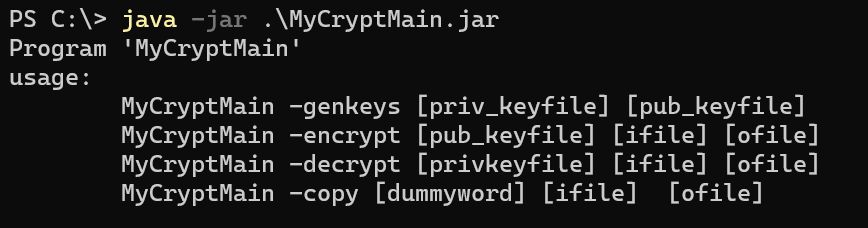
\includegraphics{./img/basic}
	\captionof{figure}{\label{fig:basic}MyCrypt Menü}
\end{center}
Das Java Programm wurde als Semi.jar kompiliert. In diesem Zustand ist es von jedem „normalen“ Betriebssystem aus startbar. Es erklärt sich von selbst, dass Objekte wie -genkeys, -encrypt, -decrypt und -copy als Optionen fungieren und einfach nur angehängt werden. \\
Die Attribute, welche in den eckigen Klammern stehen, sind zu einem Teil optional und zu einem anderen Teil erforderlich. Ich werde nun alle Optionen Schritt für Schritt erklären.

\subsection{Erzeugung von Schlüsseln}
Die Option -genkeys ist für die Schlüsselverwaltung zuständig. Sie hat zwei Attribute, welche den Pfad zu dem Schlüsselpaar angeben. Dabei ist in priv\_keyfile der Pfad zu dem privaten Schlüssel und in dem Attribut pub\_keyfile der Pfad zu dem öffentlichen Schlüssel hinterlegt. Dies sind freiwillige Angaben. Sollte einer der Pfade fehlen, wird eine entsprechende *.key Datei angelegt. Für den Privaten Schlüssel ergibt sich dann der Pfad aus der Lage der jar Datei. In dem Ordner, wo er sich befindet, werden nun die Schlüssel abgelegt. Der private Schlüssel als priv.key und der öffentliche Schlüssel als pub.key.\\ Ich empfehle für keinen Schlüssel einen Pfad anzugeben, da dies die Verwaltung einfacher macht. Die Lese und Schreibrechte in dem entsprechenden Ordner wird vorausgesetzt. Daraus ergibt sich folgende Ausgabe.\\

\begin{center}
	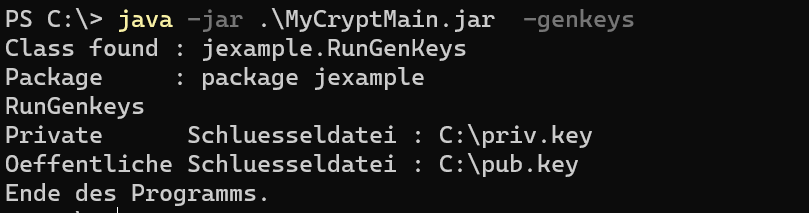
\includegraphics[width=\textwidth]{./img/genkeys}
	\captionof{figure}{\label{fig:genkeys}MyCrypt genkeys}
\end{center}

Auf die angegebene Klasse RunGenKeys sowie auf das package jexample und dessen großartigen Namen werde ich später noch genauer eingehen. Die Ausgabe suggeriert dem Nutzer den Pfad, wo die Schlüssel abgelegt werden. Als kleine Info: Die Schlüssel werden auf BASE64 gespeichert, was das Öffnen etwas lustig macht. Man kann sich den Schlüssel nicht einfach als Wert oder String vorstellen, sondern mehr als abstraktes Gebilde. Eine tiefgreifendere Bearbeitung der Schlüssel ist auf Grund des begrenzten Umfanges der Seminararbeit nicht möglich. \\


\subsection{Verschlüsseln von Datein}
Die zweite Option ist die –encrypt, welche für die Verschlüsselung zuständig ist. Dazu benötigt sie den öffentlichen Schlüssel, welcher als pub\_keyfile bezeichnet wird. Diese Angabe ist für die Verschlüsselung zwingend erforderlich. Die ifile, besser bekannt als Inputfile, bezeichnet die Datei, die verschlüsselt werden soll. Das der Pfad zu dieser angegeben werden muss, liegt ebenfalls auf der Hand. Dabei ist es irrelevant, in welchem Datentyp die Datei vorliegt.\\
 Das ofile steht an dieser Stelle für die Outputfile. Die Angabe von diesem Wert ist obligatorisch und es steht dem Nutzer somit frei, einen Eintrag zu tätigen. Sollte keine Eingabe gemacht worden sein, erfolgt die Ausgabe in einer encr\_outp.dat Datei. Dat steht hier als Dateiendung für Datei.\\


\begin{center}
	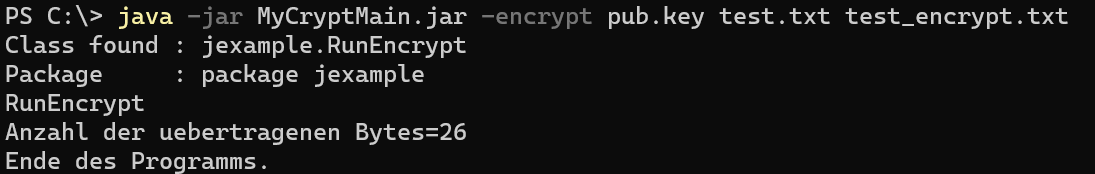
\includegraphics[width=\textwidth]{./img/encrypt}
	\captionof{figure}{\label{fig:encrypt}MyCrypt encrypt}
\end{center}
Hier fällt auf, dass zwar dasselbe Package genutzt wurde, jedoch eine andere Klasse. Grundlegend kann man sagen, dass je nach Befehl, eine andere Klasse genutzt wird. Näheres dazu werde ich später kurz beschreiben. Das Programm gibt uns die Anzahl der Bytes an, die übertragen wurden. In unserem Fall wären das 54 Bytes. Da die Datei sehr klein ist, geht auch die Datei sehr schnell von statten. Danach erfolgt wieder die Beendigung des Programmes, denn für jeden anderen Auftrag muss ein anderer Befehl genutzt werden. \\

\subsection{Entschlüsseln von Datein}
Wie bereits aus der Arbeit hervorgegangen ist, wird zum Entschlüsseln der private Schlüssel genutzt, welcher ebenfalls angegeben werden muss. Ich empfehle ausdrücklich, auch hier alle Attribute mitzuführen, da ich mir so aussuchen kann, unter welchem Namen bzw. Dateiformat die entschlüsselte Datei gespeichert wird. Bei dieser Funktion ist die Input Datei, die Datei, welche bereits verschlüsselt wurde.\\


\begin{center}
	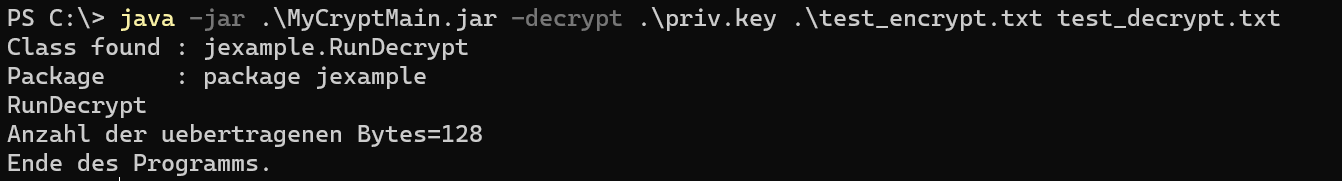
\includegraphics[width=\textwidth,height=4cm]{./img/decrypt}
	\captionof{figure}{\label{fig:decrypt}MyCrypt decrypt}
\end{center}

Nach dem erfolgreichen Aufruf dieser Methode wird die Datei wieder entschlüsselt. Dabei werden mehr Bytes übertragen als bei der Verschlüsselung.
In der Datei test.txt befindet sich derselbe Inhalt wie in der Datei test\_decrypt.txt. Es ist selbsterklärend, dass, wenn ich eine Datei mit einem öffentlichen Schlüssel verschlüssele, auch den dazugehörigen öffentlichen Schlüssel nutze, um die Datei wieder zu entschlüsseln.

\subsection{UML - Diagramm}
\begin{center}
	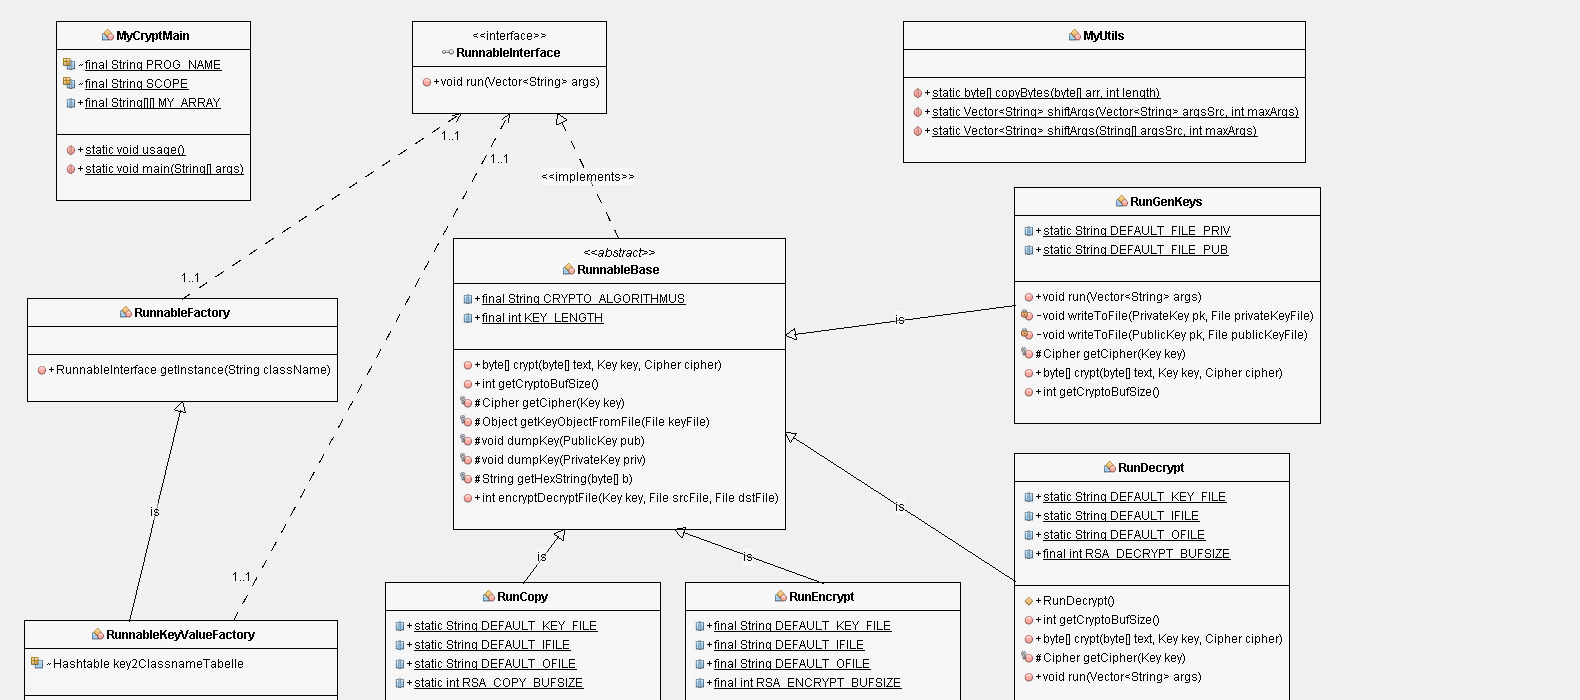
\includegraphics[width=1\textwidth]{./img/UML}
	\captionof{figure}{\label{fig:uml} UML Diagramm}
\end{center}

%% Ronny %%
\chapter{Ziele der Kryptologie}
Die Ziele der Kryptologie sind klar definiert, man spricht von drei bis vier Hauptzielen um Daten, Nachrichten und Übertragungskanäle geheim zu halten. Das erste Ziel der Kryptologie, sind die „Vertraulichkeit und Zugriffsrechte“, es bedeutet das nur autorisierte Personen Zugriff auf die Daten beziehungsweise in Computernetz versendete Nachrichten haben sollen, um private Daten oder Nachrichten lesen zu können. Anders formuliert, die Geheimhaltung einer Nachricht sollte erhalten werden. Das zweite Ziel ist die Integrität, also der Änderungsschutz, hierbei müssen alle Daten nachweislich vollständig und unverändert beim Empfänger ankommen. Das dritte Ziel ist die „Authentizität, Fälschungsschutz“, wichtig ist hier das der Urheber, also der Sender, eindeutig auf seine Nachricht identifizierbar ist, eine Fälschung der eigenen Identität also ausgeschlossen werden kann. Das bedeutet der Empfänger muss überprüfen können ob die Nachricht wirklich von dem Urheber stammt. Dieses Ziel ist schwer zum dritten Ziel zu unterschieden. In vielen Fachbüchern wird deshalb Authentizität und Verbindlichkeit unter einem Ziel zusammengefasst. Auch ich werde die Verbindlichkeit nicht explizit weiter behandeln und es auch zusammenfassend in das dritte Ziel integrieren, Grund hierfür ist unter anderem der „Platzmangel“ der Seminarfacharbeit. Das bedeutet hier wird das vierte Ziel nur Vollständigkeitshalber angesprochen, aber im weiterem Verlauf nicht weiter erläutert. So wird sich ausschließlich auf die ersten drei Ziele konzentriert. Um diese Ziele der Kryptologie erreichen zu können, und somit die Datensicherheit gewährleisten zu können, gibt es verschiedenste Methoden die wir im Vortext bereits erwähnt haben und auch in der Praxis Anwendung finden. Die Umsetzung wird fast ausschließlich durch mathematische Methoden, wie z.B. der Prüfsummen und technischen Funktionen umgesetzt. Die Ziele werden im Kapitel „Zusammenfassung“ auf unser Programm angewendet und näher erläutert. Bevor ich aber die Ziele der Kryptologie auf das RSA Verfahren anwenden kann, benötigen wir vorerst einen erweiterten Kenntnisstand über das RSA Verfahren. Ebenso benötigen wir das Wissen, wie mit Hilfe von Zielen der Kryptologie auch Datensicherheit gewährleistet werden kann. 

\section{Datenschutz und Datensicherheit}
Datenschutz ist eng mit der Kryptologie verbunden, weil sie ähnliche Ziele verfolgen. Anders formuliert, die Kryptologie wird verwendet um Datensicherheit gewährleisten zu können. Der allgemeine Grundsatz der Datensicherheit lautet, „Datensicherheit ist der Schutz von Daten vor Verfälschung, Zerstörung oder Verlust.“, Datenschutz hingegen beschäftigt mit dem Schutz des Persönlichkeitsrechts bei der Datenverarbeitung. Grundsätzlich sagt er aus, dass jeder selbst für seine Daten verantwortlich ist und selber entscheiden kann wen er welche Daten anvertraut. Der Datenschutz bezieht sich also eher auf die rechtlichen Aspekte, die im Kapitel „Kryptographie in Recht und Gesellschaft“ näher erläutert werden. Die Datensicherheit ist also grundlegender und für den technischen Aspekt wichtiger.\\

Hierbei kann die Datensicherheit durch Virenprogramme, Firewall, Passwortabfrage, aber natürlich auch mit den allgemeinen Verschlüsselungen erhalten werden. Verwendet werden diese Maßnahmen für Datenschutz und Datensicherheit um vor Viren, Würmer oder Trojanern schützen zu können. Die Vorbeugung solcher Angriffe bietet unter anderem auch die Kryptographie. Damit beispielsweise ein Fremdzugriff durch Trojaner auf die privaten Daten erschwert wird und ein sicherer Austausch von Daten gewährleistet werden kann. Es gibt somit verschiedenste Möglichkeiten seine Daten verschlüsseln zu können, um Fremdzugriff verhindern zu können. Die Verschlüsselung wird dennoch in unserer Seminarfacharbeit ausschließlich mit asymmetrischen Verschlüsselungen veranschaulicht und angewandt. Anzumerken ist aber, dass es natürlich noch andere Möglichkeiten gibt, z.B. durch die symmetrischen Verschlüsselungen Datensicherheit zu erreichen. \cite{Sicherheit}\\

\section{Ziel 1 und 2 der Kryptologie}
Um die Ziele der Kryptologie in Bezug auf die RSA Verschlüsselung beschreiben zu können, benötigt es ausführliches Wissen über den RSA Algorithmus. Alle Grundlagen des RSA Verfahrens wurden bereits im vorherigen Kapitel „Asymmetrische Verschlüsselung“ ausführlich erläutert. Der folgende Inhalt bezieht sich auf die Grundlagen der asymmetrischen Verschlüsselung.\\

Nun kann mit Hilfe des RSA Algorithmus Schlussfolgerungen für die Datensicherheit gezogen werden. Es gilt also zu klären, ob der RSA Algorithmus die Ziele der Kryptologie erfüllt. Um nun die Tauglichkeit der RSA zu überprüfen, wenden wir die bereits genannten 3 Ziele der Kryptologie an, finden tut man diese im Kapitel „Ziele der Kryptologie“. Nun mehr zur theoretischen Überprüfung der Ziele. Das erste Ziel wird klar erfüllt, denn nur berechtigte Personen haben die Möglichkeit auf eine RSA Verschlüsselung zuzugreifen, indem sie entweder „d“ wissen, oder einfach ausgedrückt „p1“ und „p2“ wissen. Der private Schlüssel ist also nur einsichtig für berechtigte Personen. Das bedeutet die Geheimhaltung wäre gewährleistet, da nur der Empfänger die verschlüsselte Nachricht einsehen kann. Ebenso ist zu empfehlen „p“ und „q“ nach der Schlüsselerzeugung zu vernichten, da nur mit ihnen eine Rekonstruktion des Schlüsselpaares möglich ist. Das zweite Ziel wird auch erfüllt, weil hier die eigentliche Zahl „d“ nicht verändert werden kann, außer man kennt als Dritter „p1“ und „p2“, dann wäre eine Veränderung von „d“ möglich und das Endergebnis wäre veränderbar. Aber um „d“ verändern zu können, benötigt der Angreifer entweder „n“, oder „p1“ und „p2“ und das ist sehr schwer herauszufinden, vorausgesetzt „n“ oder „p1“, „p2“ sind nicht leicht zu faktorisieren. Das bedeutet die Nachricht kann nur vor der Verschlüsselung mit dem öffentlichen Schlüssel noch verändert werden. Eine Veränderung der Nachricht nach der Verschlüsselung ist also nicht mehr möglich, nicht einmal für denjenigen, der die Nachricht verschlüsselt hat. \\

Denn nur der Empfänger besitzt den passenden privaten Schlüssel für seinen öffentlichen Schlüssel, dass bedeutet nur er ist in der Lage die Nachricht wieder zu entschlüsseln. Dennoch um beweisen zu können, dass die Nachricht verändert wurde, wird das Ziel abseits vom eigentlichen RSA Verschlüsselungsverfahren durch Anwendung von Hashes erzielt. Im nächsten Kapitel möchte ich speziell auf die Hashfunktion eingehen, weil diese auch von mir praktisch im Form eines Programmes angewendet wird.


\subsection{Hashes}

Hashes oder auch Hashfunktionen sind essentiell wichtig für die Kryptographie. Im Rahmen unserer Seminarfacharbeit wird sich auf den Anwendungsbereich der Integrität beschränkt. Im Prinzip ist die Hashfunktion eine kryptografische Prüfsumme für eine Nachricht, um Integrität gewährleisten zu können. Zur Verdeutlichung, in der Praxis wird eine beliebige Zeichenfolge erzeugt und durch die Hashfunktion in einen Hashwert beziehungsweise Prüfsumme „umgewandelt“ und verschickt. Nun erhält der Empfänger die Nachricht mit der Zeichenfolge und auch den dazugehörigen Hashwert. Aber der Empfänger möchte sicher gehen das der Text nicht verändert wurde, so vergleicht er die beiden Hashes, also vom Sender und Empfänger. Stimmen sie überein, dann ist keine Veränderung der Nachricht erfolgt und ist somit das Original. Ist der Hashwert anders, ist beim übertragen entweder die Nachricht manipuliert worden, oder es ist zu einer fehlerhaften Übertragung gekommen. Das alles wird ermöglicht durch einen Hashwert, der möglichst von jeden einzelnen „Nachrichtenbit“ abhängt. Das bedeutet, dass durch die kleinste Veränderung in der Zeichenfolge beziehungsweise des Textes eine große Änderung im Hashwert sich widerspiegeln sollte. Kommen wir nun zu einigen weiteren Eigenschaften die eine Hashfunktion besitzen sollte. Eine Hashfunktion basiert auf sogenannten Einwegfunktionen. Das heißt sie werden nur für einen bestimmten Zeitraum zur Verfügung gestellt. Grund hierfür ist unter anderem die mögliche Kollision zwischen Hashwerten. So kann es beispielsweise vorkommen, dass es zufälligerweise zwei identische Hashwerte gibt, um das aber verhindern zu können, werden heutige Hashalgorithmen mit einer Länge mit bis zu 160 Bit ausgestattet und zeitlich begrenzt, z.B. MD5- Message Digest 5. Ebenso darf die Umkehrung einer Hashfunktion, also die Ermittlung der Nachricht zu einem gegebenen Hashwert nicht möglich sein. Wichtig ist auch zu erwähnen das der Hashwert in der Praxis separat verschlüsselt wird, da sonst eine Änderung der Hashes im Text der verändert wurde, die Gefahr besteht, dass der Hashwert angeglichen werden könnte und so eine Verfälschung der Nachricht sich nicht im eigentlichen Hashwert widerspiegeln würde. Hashes bieten also viele Vorteile die auch in der RSA Verschlüsselung ihre Anwendung finden. Nun habe ich mich dafür entschieden eine Hashfunktion auf das RSA Verfahren anzuwenden. Um mögliche beweise und Entschlüsse für RSA im allgemeinen und unseren Programmen zu verdeutlichen. \\

\subsection{Hashfunktion und deren Anwendung}
Nachdem ich mich intensiv mit der RSA Verschlüsslung und dessen mathematischen Kontexten beschäftigt habe, bin ich nun in der Lage ein Programm mit Hilfe der Programmiersprache Java zu schreiben. Voraussetzung für das volle Verständnis wird im Kapitel „Asymmetrische Verschlüsselung“ erlangt, indem sich intensiv mit den mathematischen Kontexten des RSA Verfahrens auseinandergesetzt wird. Hierbei stand im Mittelpunkt herauszufinden, ob und wie man eine Hashfunktion in einem Programm umsetzten kann, um das Ziel der Integrität gewährleisten zu können. Um damit Rückschlüsse auf die allgemeine Tauglichkeit von RSA schließen zu können. Zweitens wird in diesem Abschnitt nur das Programm erläutert. Ergebnisse werden im Kapitel „Tauglichkeitsuntersuchung“ präsentiert. Der Quelltext ist im Anhang zu finden, im nachfolgenden Text werden Zeilenangaben des Quellcodes angegeben, um alles nachvollziehen zu können. Das Programm wird in 3 Klassen untergliedert. Die Klassen Vars.java, SetFuncs.java, Hash.java. Die Klasse Vars.java legt alle Variablen fest, diese für die Implementierung des RSA Algorithmus benötigt werden. Diese lauten „p,q,N,e,c,d,M“. Die Bezeichnung der Variablen werden fast in jeder Literatur die sich mit RSA beschäftigt verwendet und auch im Anhang erläutert, unter Glossar. Hierbei werden alle Variablen auf private und „int=0“ gesetzt, außer M mit den Datentyp char. Char deswegen, weil als Veranschaulichung nur ein Zeichen verschlüsselt wird, also ein char und kein String. Ebenso werden hierfür für alle Variablen „set und get Methoden“ festgelegt. Die „set und get Methoden „werden benötigt um die einzelnen Variablen einlesen und „verwenden“ zu können. In der Klasse SetFuncs.java, hier werden alle Methoden zur Berechnung für den RSA Algorithmus implementiert. Es werden auch nicht alle Funktionen im folgenden Text ausführlich erläutert, da ich sonst den Rahmen der Seminarfacharbeit nicht einhalten könnte. Da aber jede Funktion essentiell wichtig ist, wird jede Funktion im Anhang im Quelltext nochmals kurz kommentiert. Nicht nur die Funktionen spielen einzeln wichtige Rollen. So ist es wichtig sie auch untereinander und einzeln zu überprüfen, ob sie die Bedingungen für die einzelnen Variablen erfüllen. Werden die Bedingungen nicht erfüllt, wird das Programm abgebrochen, weil der RSA Algorithmus sonst nicht „funktionell“ funktionieren würde. Das bedeutet die Funktionen gewährleisten, dass die Richtlinien mathematischer Kontexte eingehalten werden. In Zeile 26 des Quellcodes wird die Befehlssammlung für die Hashfunktion MD5 erzeugt, die für die Erzeugung des Hash benötigt wird. In Zeile 32 wird die Befehlssammlung in ein Bytearray eingelesen. In Zeile 35-39 werden Teile des Substrings mit Hilfe des Stringbuilders an diesen angehangen. In Zeile 62-70 wird die Funktion zur Berechnung des „ggT“, größter gemeinsamer Teiler, ermittelt, also „e“.Zeile 80-82 prüft mit „boolean“ ob die Bedingung des „ggT“ erfüllt werden. In Zeile 90-97 wird mit einer „for Schleife“ in der Gleichung 1=(e*d) mod ((p-1)*(q-1)) geprüft, ob ein Wert von 0-20 als „d“ in Frage kommen würde. In Zeile 110-112 wird ein „char“, also ein Zeichen beziehungsweise „M“ für die Verschlüsselung eingegeben. In Zeile 120-137 wird geprüft ob es sich hierbei um eine Primzahl oder nicht handelt, also ob es sich hierbei um eine natürliche Zahl handelt, die größer als eins und ausschließlich durch sich selbst und durch eins teilbar ist. In Zeile 144-189 finden noch weitere Überprüfungen statt, die für eine Anwendung des RSA Algorithmus benötigt werden. Das bedeutet es wird geprüft ob „e“ teilerfremd zu „p“ und „q“ ist, ebenso wird geprüft ob „p“ und „q“ nicht die gleichen Primzahlen sind. Es wird also der Zusammenhang der Variablen und Funktionen untereinander überprüft. Nun zur dritten Klasse Hash.java, die nun die Funktionen, Variablen benutzt und anwendet. In Zeile 17 wird ein Objekt erstellt was die Funktionen lädt, dass bedeutet hier findet keine Vererbung im eigentlichen Sinne statt. In Zeile 20-32 werden „p,q,e“ eingegeben. In Zeile 35 wird der private Schlüssel erzeugt, also d. In Zeile 38 wird der öffentliche Schlüssel, also „N“ erzeugt. In Zeile 41 wird eine Nachricht eingegeben, also ein Zeichen durch char, also „M“. In Zeile 47 wird nun mit den eben genannten Funktionen die Nachricht verschlüsselt. Ebenso wird „M“ vorher noch umgewandelt, vorerst in einen String und dieser dann in ein int Wert. Da „$A^24$“ nicht lösbar ist. So werden die einzelnen Zeichen mit Hilfe der ASCII Tabelle in int Werte umgewandelt. In Zeile 52 - 54 erfolgen die Ausgaben mit dem jeweiligen Hash und der verschlüsselten und entschlüsselten Nachricht. Diesen Hashwert könnte man sich vormerken und mit der veränderten Nachricht vergleichen. Um die Hashwerte vergleichen zu können, um Rückschlüsse auf eine mögliche Manipulation schließen zu können.

\subsection{Ziel 3 der Kryptologie}
Das dritte Ziel kann auch erzielt werden. Nun kann die RSA Verschlüsslung aber grundsätzlich keine Authentizität gewährleisten. Um das Problem lösen zu können, hilft sich die Kryptographie mit den sogenannten digitalen Signaturen aus. Das bedeutet jede Nachricht ist auf einen Benutzer zu 100\% zuzuordnen. Das wird ermöglicht, durch den sogenannten virtuellen Fingerabdruck. Er gibt jeder Nachricht eine individuelle Erkennbarkeit. Dabei ist wichtig das keine sichere Datenübertragung nur mit digitalen Signaturen erreicht werden kann, es ist nämlich trotzdem eine Verschlüsslung notwendig. So kommen wir zu Problemen der Authentizität bei den RSA Verfahren. Es ist nämlich nicht direkt möglich bei einer RSA Verschlüsslung herauszufinden, ob es sich beim Sender wirklich um die Person handelt, oder ob er seine Identität fälscht. Das bedeutet das Ziel der Authentizität kann vorerst nicht erreicht werden. Nun ist es aber möglich RSA im Grundprinzip auf ein Signaturverfahren „umzumünzen“. Das bedeutet es wird ermöglicht die Schlüssel zu vertauschen. Dennoch werden wir im Rahmen unserer Seminarfacharbeit nicht spezieller auf den Algorithmus des Signaturverfahrens mit RSA eingehen. Um eine digitale Signatur mit dem Prinzip der RSA erreichen zu können wird wie bereits erwähnt die Funktion der Schlüssel getauscht. So wird hierbei mit dem privaten Schlüssel verschlüsselt und mit dem öffentlichen Schlüssel entschlüsselt. Und weil der private Schlüssel bekanntlich nur einer Person zugeordnet werden kann, ist die Nachricht nachweislich zu 100\% von der Person der mit diesem privaten Schlüssel eine Nachricht verfasst hat. Dadurch wäre die Authentizität gewährleistet. Die Nachricht wird dann mit dem öffentlichen Schlüssel entschlüsselt. Nun ist hierbei die Authentizität und Integrität gewährleistet, aber nicht mehr die eigentliche Geheimhaltung. So ist es nun jeden möglich die verschlüsselte Nachricht mit dem öffentlichen Schlüssel zu entschlüsseln und zu lesen. Man kann also festhalten das das RSA Verfahren mehrere Anwendungsmöglichkeiten bietet. Zum einen kann man „geheim“ verschlüsseln und zum anderen eine digitale Signatur erstellen. Dennoch besteht auch eine sehr komplexe Möglichkeit, die ermöglicht beides gleichzeitig anzuwenden. Wir haben uns aber bewusst gegen ein Programm entschieden, welches digitale Signaturen und gleichzeitig die Geheimhaltung gewährleisten soll, weil wir sonst den fachlichen Rahmen zu weit ausgebreitet hätten und somit auch jeglichen Rahmen einer Seminarfacharbeit. Somit beschränken wir uns auf die Geheimhaltung. Es gibt auch mehrere Sicherheitsprobleme bei den digitalen Signaturen der RSA, diese auf mathematische Kontexte zurückzuführen sind, dennoch ich im Rahmen unserer Seminarfacharbeit nicht weiter ausführen möchte. Die eben genannten „komplexen“ Möglichkeiten finden ihren Anklang vor allem in der Praxis, da sie die eben genannten Vorteile mitbringen.

\section{RSA in der Praxis}
In der Praxis findet das RSA Verfahren Anklang bei den digitalen Signaturen, wie PGP, Pretty Good Privacy“ und SSH, „Secure Shell“. Hierbei werden sie oft in Form von Hybriden Verschlüsselungen angewendet, also Verschlüsselungen die zum Beispiel symmetrische und asymmetrische Verfahren kombinieren. Die RSA Verschlüsselung benötigt für große Datenmengen aber viel zu viel Zeit. Das hat zur Folge, dass die RSA Verschlüsslung nicht direkt bei Verschlüsselungen für große Datenmengen zur Anwendung kommt, sondern eher zum verschlüsseln des „kleinen“ Saison-Keys der symmetrischen Verschlüsselung. Um es kurz zu fassen, es werden Nachrichten mit großen Datenmengen, mit Hilfe des symmetrischen Verschlüsselungsverfahren verschlüsselt und weil das noch keine ausreichende Sicherheit gewährleisten würde, wird der Schlüssel der symmetrischen Verschlüsselung mit einem asymmetrischen Schlüssel zusätzlich verschlüsselt. Somit wird das langsame asymmetrische Verfahren, welches für große Daten äußerst lange braucht, nicht eingesetzt. Dafür verschlüsselt man mit dem asymmetrischen Verfahren, den Schlüssel des symmetrischen Verfahrens, da die Schlüssel nur aus kleinen Datenmengen bestehen. Abschließend ist zu sagen, dass asymmetrische Verschlüsselungen gänzlich ungeeignet sind für reine Geheimhaltungen von großen Datenmengen, sie werden meistens in Kombination mit anderen Methoden eingesetzt, weil sonst die eben genannten Nachteile überwiegen. Es gibt noch zahlreiche andere Funktion, die ich aber im Rahmen unserer Seminarfacharbeit nicht weiter aufgreifen werde.

\section{Kryptoanalyse}
Bevor ich mich mit der Kryptoanalyse beschäftige muss gesagt werden, dass ich nicht alle Angriffsmethoden nennen und erläutere. Denn nur alleine die Kryptoanalyse würde genügend Informationen für noch eine Seminarfacharbeit bieten. So gebe ich einen grundlegenden Überblick über die Kryptoanalyse und gehe auf ein Verfahren näher ein.\\

Soeben wurden Möglichkeiten aufgezeigt, wie man sich mit Hilfe von Verschlüsselungsmethoden, mit beispielsweise RSA schützen kann und somit unbefugten Personen Eintritt auf private Nachrichten verweigert werden können. Nun aber zum zweiten großen Teil der Kryptologie, die Kryptoanalyse. Diese beschäftigt sich nicht mit der Entwicklung neuer Methoden, sondern wendet schon bereits vorhandene Methoden an, um diese auf Schwachstellen abzusuchen und mögliche Sicherheitslücken finden zu können. Mit dem Ziel die verwendete Verschlüsselungsmethode zu stärken und von Sicherheitslücken befreien zu können. Anders formuliert: „Analyse und Bewertung der Sicherheit von Kryptoverfahren gegen unbefugte Angriffe“.\\

Besonders für meinen Eigenanteil ist die Kryptoanalyse sehr wichtig, weil ich in der Rolle eines Kryptoanalytiker handle und das RSA Verfahren in Bezug auf unsere Programme auf Tauglichkeit untersuche. So ist eine Tauglichkeitsuntersuchung durch einen Kryptoanalytiker besonders wichtig in der heutigen Zeit, um Schwachstellen eines Programmes vor der Veröffentlichung ausfindig zu machen. Nun kann natürlich Kryptoanalyse nicht nur zur Stärkung von Programmen genutzt werden, sondern meist wird Kryptoanalyse von „Angreifern“ genutzt, die das Ziel verfolgen ein verschlüsseltes Programm beziehungsweise Nachricht zu entschlüsseln, indem er zum Beispiel den geheimen Schlüssel herausfindet. Aber auch andere Sicherheitslücken können genutzt werden, so kann es beispielsweise vorkommen, dass der Angreifer nicht einmal einen Schlüssel benötigt um an die geheimen Informationen zu kommen. Das wäre das sogenannte „Worse-Case“ eines Programmes und zeichnet ein nicht ausreichend getestetes Programm aus. Es gibt verschiedene Möglichkeiten um an den geheimen Schlüssel zu gelangen.\\

\subsection{Angriffsverfahren durch Kryptoanalyse}
Nun zu einigen „gängigen Methoden“. Zum Beispiel der known Ciphertext, Known Plaintext, Chosen Plaintext und Chosen Ciphertext Angriff. Aufgrund des „Platzmangels“ können die eben genannten Verfahren nicht weiter erläutert werden. Dennoch wird sich mit einer Methode näher beschäftigt und zwar mit dem Bruce-Force Angriffsverfahren. In der Bruce-Force Angriffsmethode wird versucht den Schlüssel durch schlichtes probieren zu ermitteln. Natürlich nicht mit Stift und Papier, sondern mit Computern. Heutzutage wird hierfür viel Rechenleistung benötigt, um Möglichkeiten des Schlüssels „durchzuspielen“. Ein Beispiel wäre, nimmt man einen Schlüssel mit der Schlüssellänge von 25 Bit, hätte man $2^25$ Möglichkeiten, also 33.554.432 Möglichkeiten. Nun nehmen wir an, wir bräuchten 2 Sekunden um eine Kombination eines Schlüsselpaares auszuprobieren. Man bräuchte also maximal ca. 776 Tage, also ca. 2 Jahre bis man alle Möglichkeiten ausprobiert hätte und somit auch zu 100\% den Schlüssel hätte. Wichtig hierbei anzumerken ist, dass auch gleich beim ersten Versuch der Schlüssel gefunden werden könnte, oder auch erst beim letzten. Des Weiteren werden in der Praxis abseits von den theoretischen Methoden natürlich vor allem trojanische Pferde benutzt um an bestimmte geheime Schlüssel zu gelangen, aber auch kann man jemanden gezielt ein geschwächtes Verschlüsselungsverfahren „anvertrauen“, um daraus seinen Erfolg zu erzielen. Zum Beispiel ein Programm entwickeln, welches mit Sicherheitslücken an eine Organisation weiterverkauft wird. Die Kryptoanalyse bietet somit viele Möglichkeiten um Verschlüsselungen zu umgehen. Alles was man im Prinzip braucht, ist Geduld, ein „Verfahren“, Rechenleistung und natürlich auch ein wenig Glück. Hierbei möchte ich den Begriff Rechenleistung und deren Bedeutung noch einmal näher erläutern. In den letzten Jahren sind die Computer immer schneller geworden.\\
Nun erschwert folgendes Szenario die Verschlüsselungsmethode der RSA, mit der wir uns auch im Eigenanteil intensiv beschäftigen. Wie wir bereits geklärt haben, besteht diese Verschlüsselungsmethode im Prinzip auf der Geheimhaltung zweier Primzahlen. Nun könnte man aus der Sicht eines Kryptoanalytikers durch „probieren“ die Primzahlen ermitteln. Das geht natürlich umso schneller, desto schneller auch der Computer rechnen kann. Das bedeutet, wenn die Rechenleistung von Rechnern stetig steigt, müssen natürlich auch die Primzahlen größer werden.

\subsection{Brute-Force Angriffsmethode und deren Gefahren}
Im Kapitel „Angriffsverfahren durch Kryptoanalyse“ wurde geklärt was ein Bruce-Force Angriff ist und welche Gefahren entstehen können. Nun möchte ich zur Verdeutlichung meines zweiten Programmes, welches das Bruce-Force Verfahren veranschaulicht, den mathematischen Hintergrund kurz beleuchten. In dieser Erläuterung geht es um das Problem von zu klein gewählten Primzahlen in einer RSA Verschlüsselung. Grundsätzlich ist eine Veränderung der Verschlüsselung der RSA-Methode nur möglich, wenn der Wert „d“ bekannt ist, somit gibt es natürlich Möglichkeiten diesen herauszufinden. Man kann durch bestimmte Software, z.B. mein Programm, den privaten Schlüssel ermitteln. Denn sind „p1“ und „p2“ ermittelt worden, kann man „n“ errechnen und mit Hilfe von „n“ kann man „d“ errechnen. Wichtig anzumerken ist noch, dass unser Programm grundsätzlich auf kleinen Primzahlen beruht, also selbst durch vorhandene Software „relativ“ schnell eine Lösung gefunden werden kann. Das bedeutet um zu verhindern, dass man das Produkt von „n“ herausfindet, nimmt man Zahlen die nicht leicht zu faktorisieren sind. Um ein Beispiel zu nennen, $p1=2^30$, $p2=2^35$, nun soll man aus diesen beiden Faktoren das unbekannte Produkt „n“ finden, weil ja n=(p1-1) *(p2-1), hier wird es den Angreifer um einiges schwieriger gemacht das Produkt „n“ zu finden um später „d“ ermitteln zu können. Aus diesem Grund ergibt sich ein Richtwert für Schlüssellängen. So ist für einen asymmetrischen Schlüssel mindestens eine Länge von 1024-2048 Bit oder 3072 Bit zu wählen. Für die längerfristige Sicherheit sollten die Schlüssel eine Länge von 15360 Bit haben. Man kann also festhalten, dass der Bruce-Force Angriff durch die massive Rechenleistung, bei Verschlüsselungssystemen mit kurzen Schlüsseln eine echte Bedrohung darstellt. Ausschließlich mit langen Schlüsseln kann man sich gegen die Bruce-Force Angriffe schützen. Der Bruce-Force Angriff eignet sich also ideal um eine Schwachstelle der RSA zu veranschaulichen. Deswegen habe ich mich dazu entschieden die Bruce-Force Angriffsmethode und deren Gefahren für das Verschlüsselungsverfahren der RSA, mit Hilfe eines „Demo Programms“ zu beweisen.

\subsection{Bruce-Force Programm}
Die Simulation des Bruce-Force Programms erfolgt ebenso in einem Java Programm, was ganz normal von Netbeans ausgeführt werden kann. Die Erstellung des RSA Algorithmus ist identisch zum Hash Programm und wird somit in das Programm übernommen. Das „Demo Programm“ arbeitet mit einer festgelegten „size“, die auf genau 4 Bit festgelegt ist. Nun werden Eingaben von „p“, „q“ und „e“ abgefragt, die von einem Benutzer eingegeben werden sollen um schlussendlich damit ein Zeichen „m“ zu verschlüsseln. Im Programm wird versucht „p“ und „q“ zu errechnen um „n“ errechnen zu können. Wenn „p“ und „q“ ermittelt worden sind, kann nun damit ohne Probleme „d“ errechnen werden. Im Programm wird die Ermittlung mit zwei „verschachtelten „for Schleifen““ umgesetzt. Das bedeutet der jeweilige „x“, „y“ Wert wird nacheinander erhöht, bis die passenden Primzahlen, die eingegeben Primzahlen gefunden worden sind.

\section{Tauglichkeitsuntersuchung}
Erarbeitung des Eigenanteils aus Sicht eines Kryptoanalytikers. Dabei gehe ich wie folgt vor. Ich werde das erarbeitete theoretische Wissen, durch die Literatur, praktischen Anwendungen und durch selbst entwickelte Programme zusammenfassen und eine „Tauglichkeitstabelle“ ausarbeiten. Ziel der Tabelle ist es, den Nutzer erstens schnell einen Überblick über die wichtigsten Merkmale der Verschlüsselung zu vergegenwärtigen und zweitens Programme auf die Tabelle anwenden zu können, umso eventuell Schwachstellen für seinen eigenen Algorithmus finden zu können. Also unseren eigens programmierten Algorithmus auf Tauglichkeit zu testen. Die Tauglichkeitsuntersuchung wird in verschiedene Bereiche untergliedert, auf die die Tauglichkeitstabelle wie eine Checkliste angewendet wird. Nach der Untersuchung der Tauglichkeit der einzelnen Bereiche, wird eine Gesamtwertung der Programme erfasst und ausgewertet. Die Tabelle wird nicht alle Themengebiete die erarbeitet worden sind abdecken, da wir sonst den Rahmen der Seminarfacharbeit „sprengen“ würden. Es ist zu erwähnen das alles, was in der Tabelle verwendet wird, nicht auf alle Verschlüsselungen sinnvoll und logisch ist. Die Tabelle bezieht sich also grundsätzlich auf die asymmetrische Verschlüsslung, wie das RSA Verfahren. Ebenso ist alles sehr theoretisch und in der Praxis nicht immer umsetzbar und logisch. Dennoch werden mit zwei Programmen auch praktische Anwendungen veranschaulicht. Um aber in der Lage zu sein, eine Tauglichkeitsuntersuchung des Verfahrens der RSA von einem selbst erstellten Programm durchführen zu können, benötigen wir das Wissen aus den bereits erarbeiteten Kapiteln, speziell die Ziele der Kryptologie, Schwachstellen durch Kryptoanalyse und ausführliches Wissen über das Verfahren der RSA. \\
Zu Anfang kann ich festhalten, dass eine Verschlüsslung in der Lage sein sollte, so viele Ziele der Kryptologie wie möglich gewährleisten zu können. Um die Datensicherheit garantieren zu können. Ebenso sollte eine Verschlüsslung einen brauchbaren Schutz vor Angreifern und Schutz vor den gängigsten Angriffsmethoden haben. So werden folgende Bereiche bei der Tauglichkeitsuntersuchung mit einfließen. Die drei Ziele der Kryptologie, die Kryptoanalyse durch das Bruce-Force Angriffsverfahren veranschaulicht, ebenso werden praktische Aspekte mit aufgeführt. Aber vorher ist noch wichtig anzumerken, dass es sich zwar primär um unser Hauptprogramm handelt, dass das RSA Verfahren anwendet, dennoch ich Teilprogramme bilden musste. Ich habe mich also entschieden sogenannte „Demo-Programme“ zu erstellen. Der Grund ist die Komplexität des Hauptprogramms, die wir überschreiten würden, wenn wir keine Auslagerungen des Hauptprogramms durch „Demo Programme“ vorgenommen hätten. Das bedeutet wir hätten den Rahmen unserer Seminarfacharbeit mehrfach überschritten. Ebenso ermöglichen mir die „Demo Programme“ einzelne bestimmte Aspekte verdeutlichen und beweisen zu können, in Bezug auf die „Tauglichkeitsuntersuchungen“ des RSA Verfahrens. Weitere inhaltliche Gründe für die Auslagerung vom Hauptprogramm finden sie im fortlaufenden Text. Beginnen wir nun mit den Zielen der Kryptologie. Ich kann die Ziele der Kryptologie mit Hilfe der Programme und theoretischen Wissen über das RSA Verfahren beweisen und widerlegen. So habe ich unseren Algorithmus, der auf der Grundlage der RSA Verschlüsslung arbeitet, intensiv getestet. So bin ich diesbezüglich zum Entschluss gekommen, dass unsere Programme manche Ziele erfüllen und andere wiederum nicht. Hierbei gibt es keinerlei Abweichung zum theoretisch erarbeiteten Wissen, welches bereits im Kapitel „Ziele der Kryptologie“ erarbeitet und ausführlich erläutert wurde. Dort wurde erläutert wieso und weshalb manche Ziele erreicht und andere nicht erreicht werden können, dieser Erkenntnisgewinn spiegelt sich voll und ganz in unseren Programmen wieder und kann somit von mir bewiesen werden. So habe ich festgestellt, dass das erste Ziel der Kryptologie, was besagt das alle Daten nur von autorisierten Personen gelesen werden können, erfüllt wird. Das erste Ziel wird erfüllt, weil unser Programm auf der Grundlage der RSA Verschlüsselung arbeitet und so in der Lage ist einen Text sicher zu verschlüsseln, also der Text ohne privaten Schlüssel nicht zu entschlüsseln ist, somit ist die Geheimhaltung gewährleistet. Des Weiteren habe ich festgestellt, dass auch das zweite Ziel der Kryptologie, was besagt das alle Daten beim Empfänger unverändert seien müssen, erfüllt ist. Hierbei ist aber wichtig anzumerken, dass das Ziel theoretisch bereits dadurch erfüllt wird, weil die RSA Verschlüsslung es mathematisch kaum ermöglich die Primzahlen herauszufinden, wenn sie denn groß genug sind. Dennoch kann ich zusätzliche Beweise liefern. Bewiesen wird es durch ein Hilfsprogramm, was sogenannte Hashes von MD5 verwendet, dass ausführlich erläutert worden ist. So wird es ermöglicht jede Nachricht mit einem Hashwert auszustatten. Das bedeutet jede Nachricht ist abhängig von jedem einzelnen Bit der Nachricht. \\
Durch mehrere Tests des Programmes wurde festgestellt, dass die kleinste Veränderung einer Nachricht eine große Änderung des Hashwertes widerspiegelt und eine Manipulation der Nachricht somit bewiesen werden kann. Voraussetzung hierfür war, den Hashwert der Nachricht vom Sender zu notieren und ihn nach der Ausführung der Verschlüsselung mit diesen zu vergleichen. Da jedes Zeichen einen anderen Hashwert hat, beweist, dass eine veränderte Nachricht auch einen anderen Hashwert haben würde. Das heißt wir konnten nicht während der Verschlüsselung den Hashwert überprüfen, dass bedeutet ein realistischer Manipulationsangriff wurde nicht simuliert, dennoch würde jemand einen Angriff ausführen, würde sich nun aber die Nachricht ändern, demnach auch ein völlig anderer Hashwert entstehen. Ebenso wird bei jeder Nachricht ein neuer Hashwert generiert und eingesetzt. Es werden also die grundlegenden Richtlinien der Hashfunktionen erfüllt, diese bereits im Kapitel „Hashes“ erläutert worden sind, dennoch haben wir eine zeitliche Begrenzung der einzelnen Hashwerte nicht eingebaut. Die Funktion würde keinerlei Sinn ergeben in unseren „Demo Programm“, denn doppelte Hashwerte im Bereich von 160 Bit sind extrem unwahrscheinlich. Würde man das „Demo Programm“ jedoch im „World Wide Web“ anbieten, müsste natürlich aus Sicherheitsgründen eine zeitliche Begrenzung der einzelnen Hashwerte erstellt werden. So kann man festhalten, dass Hashfunktionen für die Integrität sehr wichtig sind. Denn sie sorgen dafür das Manipulationen unabhängig von der eigentlichen „Schutzfunktion“ der RSA Methode nochmals abgesichert werden und zeitgemäß geschützt werden können. Kommen wir nun zum dritten Ziel der Kryptologie, dass besagt das eine Nachricht eindeutig auf eine Person zurückzuführen ist. Das Ziel kann durch unser Programm nicht erreicht werden, aber auch nicht in der Theorie. Außer die Funktion wird durch den bereits erläuterten Schlüsseltausch oder Hybride Verschlüsselungen ermöglicht. Hierbei ist besonders wichtig zwischen zwei Varianten der RSA Verschlüsslung zu unterscheiden. Denn entweder man verschlüsselt seine Nachricht mit dem Verfahren, wie wir es erläutert und umgesetzt haben oder aber man benutzt den RSA Algorithmus, um eine digitale Signatur zu erstellen, um das dritte Ziel erfüllen zu können. Dabei hat alles seine Vorteile und Nachteile die bereits erläutert wurden. Da wir uns aber auf die allgemeine RSA Verschlüsslung konzentriert haben, kann das Ziel leider nicht erreicht werden. Nun kommen wir zu einem wichtigen Teil der Kryptologie und zwar zur Kryptoanalyse. Ich habe mich entschieden die Bruce-Force Angriffsmethode und deren Gefahren auf die RSA Verschlüsslung virtuell mit Hilfe eines weiteren „Demo Programms“ zu beweisen. Auch hier musste wieder eine Auslagerung vom eigentlichen Hauptprogramm vorgenommen werden. Grund ist, weil unserer Hauptprogramm ausschließlich nur mit abstrakten Klassen und Zahlen arbeitet, also nur zur Veranschaulichung des RSA Algorithmus. \\
Um aber mit Zahlen arbeiten zu können, um die Berechnung der Primzahlen zu ermöglichen, musste ich eine Auslagerung des Hauptprogramms vornehmen, die ich zur Veranschaulichung des Bruce-Force Angriffsverfahren essentiell benötige. Mit dem zweiten „Demo Programm“ ist es gelungen, dass Bruce-Force Angriffsverfahren simulieren zu können, dabei bin ich zu folgenden Entschlüssen gekommen. Die Bruce-Force Angriffsmethode ist zwar eine simple Methode, aber trotzdem eine der gefährlichsten Angriffsmethoden in Bezug auf RSA Verschlüsselungen mit kleineren Primzahlen, wie es im „Demo Programm“ der Fall ist. So stellt das Bruce-Force Verfahren eine große Gefahr dar und mit Hilfe des „Demo Programms“ kann bewiesen werden, dass das RSA Verfahren mit kleinen Schlüsseln leicht zu knacken ist. So können kleine Schlüssel, von 1 bis 4 Bit binnen weniger Stunden oder Tagen errechnet werden und so steht einer Manipulation der Nachricht nichts mehr im Wege. Anzumerken ist, dass es sich hier um einen Rechner mit eher mittelmäßiger Rechenleistung handelte, dass bedeutet die Berechnung von „p“ und „q“ würde mit anderen Rechnern durchaus schneller gehen. Die Tests konnten „innerhalb von Java“ nur bis 32 Bit getestet werden, weil Java nur bis zu 32 Bit, das entspricht der Dezimalzahl 2147483647, des Datentyps Integer unterstützt. Nochmals anzumerken ist, dass das Problem nicht mehr besteht, sobald größere Schlüssel verwendet werden. So wie bei unseren Hauptprogramm, welches eine Schlüssellänge von 1024 Bit beinhaltet. So ist statistisch gesehen unser Hauptprogramm zeitgemäß geschützt. Eine 2048 Bit Schlüssellänge, welches sicherer und zukunftssicherer wäre, haben wir nicht eingesetzt. Der Grund ist simpel, wir hätten durch die Berechnung eines solchen Schlüssels und mit der Verschlüsselung eines Textes ein vielfaches der Zeit benötigt. Abschließend kann festgehalten werden, dass das zweite „Demo Programm“, was die Bruce-Force Angriffsmethode simuliert, beweist, dass zu kleine Primzahlen zu einem erheblichen Sicherheitsrisiko, in der Verschlüsselung mit dem RSA Verfahren, beitragen würde. So kann abschließend festgehalten werden, dass die Programme sich verhältnismäßig gut schlagen. So werden die ersten beiden Ziele der Kryptologie erzielt und garantieren damit die Geheimhaltung der Texte, sowie die Integrität. Was zwar für Anwendungen in der Praxis eher schlecht ist, welches im Kapitel „RSA in der Praxis“ bereits beschrieben wurde, aber für unsere Seminarfacharbeit, die sich auf effektive Verschlüsselung und Geheimhaltung konzentriert völlig akzeptabel ist. So ist es möglich einen beliebigen Text einer Datei effektiv zu verschlüsseln, ebenso durch das „Hash Demo Programm“ wird noch die Absicherung durch die bereits genannten Hashes ermöglicht, welches ermöglicht die kleinste Änderung in einer Nachricht effektiv sichtbar zu machen. Dieses Programm arbeitet zwar unabhängig vom Hauptprogramm, könnte aber dennoch sofort in das Hauptprogramm integriert werden. Grund das es nicht integriert ist, ist die Komplexität des Hauptprogramms die einen Rahmen der Seminarfacharbeit „sprengen“ würde. \\
So erfüllt unser Hauptprogramm alleinstehend nicht „perfekt“ das zweite Ziel der Kryptologie, dennoch aber durch die Ergänzung des „Demo Programmes“ für Hashes, wird das Ziel unter „Vermerk“ komplett und souverän erfüllt. Es ist also gelungen den Algorithmus der RSA in Java-Code umzusetzen und so viele Ziele der Kryptologie, wie es ein Rahmen der Seminarfacharbeit erlaubt, zu erfüllen um Datensicherheit gewährleisten zu können. Ebenso beweise ich als aktiver Kryptoanalytiker, dass unser Programm einen Bruce-Force Angriff standhalten würde. Indem ein „Angriff“ mit dem Bruce-Force Verfahren simuliert wurde um zu beweisen, dass die Gefahr ausschließlich von kleinen Schlüssellängen ausgeht. Da unser Programm aber mit einer ausreichenden Schlüssellänge arbeitet, ist das Programm dahingehend sicher. Um zum Schluss zu kommen. Die Programme eignen sich nicht in der Praxis. Die Geheimhaltung und Integrität wird zwar erfüllt, was für eine Verschlüsselung ohne Authentizität ausreichend wäre, also für Nachrichten die keine große Priorität hätten. Dennoch würden sie einfach viel zu lange benötigen um einen Text, mit großer Datenmenge, erfolgreich zu verschlüsseln, auch wenn schon alles dafür getan wurde um Zeit bei der Verschlüsselung zu sparen. Indem die Schlüssellänge auf 1024 Bit begrenzt worden ist. Die einzige Aushilfe würden Hybride Verschlüsselungen bieten, mit denen man auch Authentizität gewährleisten könnte, diese aber aus Gründen der Komplexität nicht zur Anwendung kommen. Einen zusammenfassenden Überblick über die eben genannten Schlussfolgerungen der Tauglichkeit in Bezug auf die Programme finden sie im Abbildungsverzeichnis unter „Abbildung 3“ oder unter der Tauglichkeitstabelle. Ebenso ist wichtig zu erwähnen, dass ich die Seitenzahl leider nicht einhalten konnte, weil eine Tauglichkeitsuntersuchung mit wenigeren Aspekten, als ich aufgeführt habe, nicht aussagekräftig genug wäre. Ebenso ist zu erwähnen, dass bereits intensiv gekürzt worden ist. Eine weitere Kürzung würde also den inhaltlichen Rahmen zerstören und nicht aussagekräftig machen.

\begin{center}
	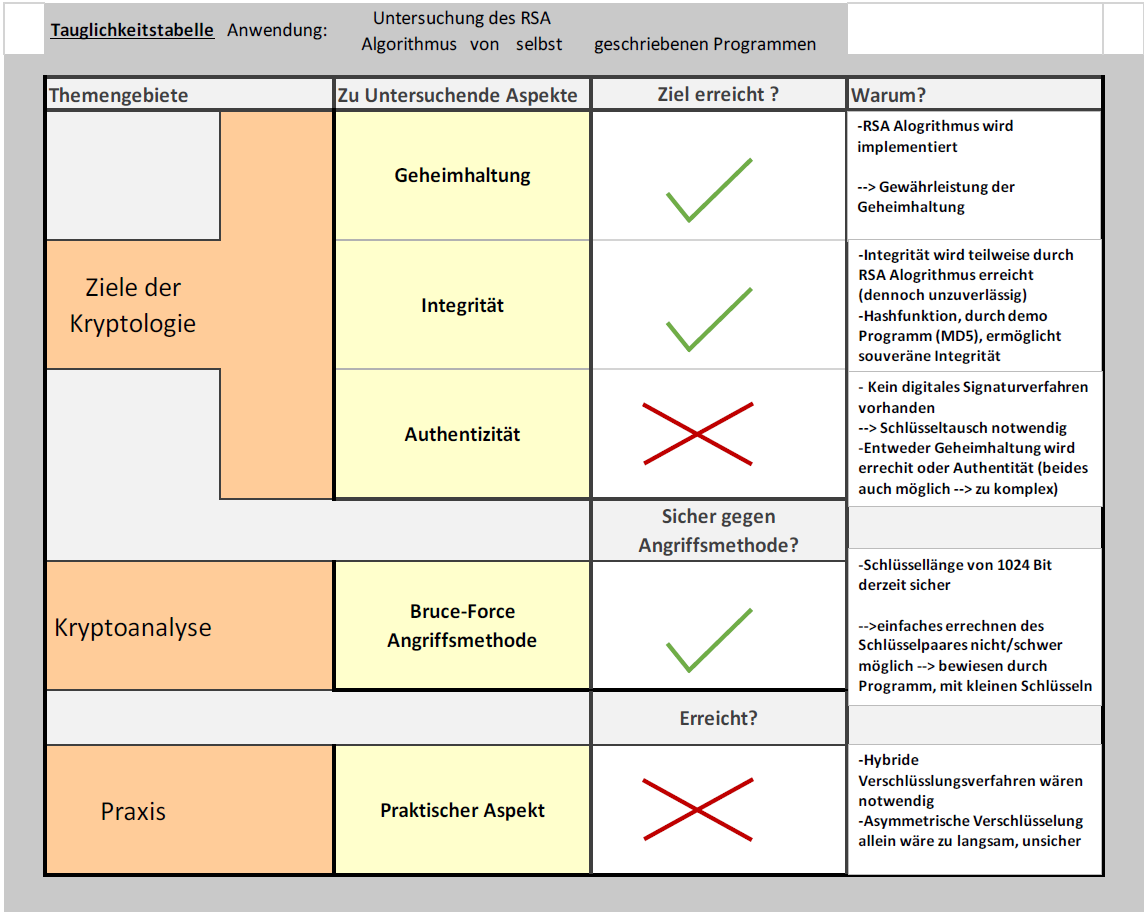
\includegraphics[width=1\textwidth]{./img/tauglichkeit}
	\captionof{figure}{\label{fig:tauglichkeit} Tauglichkeitsanalyse}
\end{center}

%% Liane %%%
\chapter{Kryptographie in Recht und Gesellschaft}
Nachdem wir uns mit der Geschichte, Verschlüsselungsverfahren und explizit mit der RSA Verschlüsselung und deren Sicherheit beschäftigt haben, kommen wir nun zu den rechtlichen Rahmenbedingungen. Sie sind besonders wichtig in Bezug auf das Kapitel „Datenschutz und Datensicherheit“ zu nennen. \\

In der heutigen modernen Zeit findet man Sie überall, die Verschlüsselung. Sei es bei Sozialen Netzwerken oder bei Smartphones. Doch wie sieht es in den Bereichen Recht und Gesellschaft aus?

\section{Rechtliche Aspekte}
\subsection{Situation in den USA}

In den USA ist es bis jetzt nicht gesetzlich geregelt, ob die Benutzung leistungsfähiger kryptographischer Verfahren strafbar ist oder nicht. Bisher unterliegt solche Hard- und Software besonderen Exportbeschränkungen und werden wie Munition behandelt. Deshalb sind für den Vertrieb in andere Länder, nur Verfahren zugelassen die maximal eine Schlüssellänge von 40 Bit besitzen. Doch diese verfahren können sehr leicht und schnell geknackt werden.

\subsection{Situation in Dänemark}
In Dänemark wird das Recht auf Verschlüsselung nicht durch ein Gesetz eingeschränkt, denn dort hat jeder das Recht darauf seine persönlichen Daten zu verschlüsseln. Wenn Firmen die Kryptographie als Grundsatz ihrer Dienste sehen, müssen Sie die Verschlüsselung, durch einen Gerichtsbeschluss entschlüsseln. Da der dänische Technologierat festgestellt hat, dass ein gänzliches Verbot von Verschlüsselungssystemen gegen den Artikel 8 und Artikel 10 der Europäischen Menschenrechtskonvention verstößt. Somit sollten Behörden keinen Zugriff auf die Schlüssel der Programme erhalten.

\subsection{Situation in Deutschland}
\subsubsection{Die Aktuelle Rechtslage}
Authentikations- und Konzelationssystemen werden im deutschen Gesetzgeber getrennt bestrafft, obwohl beide Systeme kryptographische Verfahren sind. Während das Authentikationssystem eine detaillierte gesetzliche Regelung besitzt, so ist das Konzelationssystem kaum bis gar nicht gesetzlich geregelt. Die Unterscheidung von Signatur- und Verschlüsselungsverfahren entsteht dadurch, dass sie aus juristischer Sicht verschiedenen Zielen dienen und das die Erwartungen der einzelnen Benutzern an die Systeme aus unterschiedlichen Problemen zusammensetzen.


\subsubsection{Die Gesetzgebungskompetenz}
Die Zuständigkeit der Gesetzgebung ergibt sich aus der Kompetenz des Bundes zu konkurrierenden Gesetzen der Wirtschaft (Art.74 Abs. 1 Nr. 11 GG). Damit in gesamt Deutschland die gleichen Sicherheitsbedingungen und Sicherheitsanforderungen herrschen können, ist die Einheit von Recht und Wirtschaft durch eine bundesgesetzliche Regelung gewahrt (Art. 72 Abs. 2 GG).

\subsubsection{Das Signaturgesetz}
Das Gesetz zur Behandlung der Rahmenbedingungen für Informations- und Kommunikationsdienste (Informations- und Kommunikationsdienste-Gesetz, IuKDG) vom 22. Juli 1997 enthält im Art. 3 das Gesetz zur digitalen Signatur (Signaturgesetz, SigG). Dieses Gesetz ist nach dem Art. 11 IuKDG am 1. August 1997 in Kraft getreten.

\subsubsection{Gesetzeszweck}
Die Absicht des SigG ist es, Rahmenbedingungen für digitale Unterzeichnungen zu befördern, unter denen diese als gewiss gelten und Fälschungen digitaler Signaturen oder Verfälschungen von unterzeichneten Daten zuverlässig diagnostiziert werden können (§ 1 Abs. 1 SigG). Veränderungen an Formvorschriften oder dem Beweisrecht wurden nicht vorgenommen, hauptsächlich wurde die digitale Signatur nicht der gesetzmäßigen Schriftform (§ 126 BGB) gleichgestellt. Es soll gegenwärtig durch tatsächliche Sicherheit Vertrauen in die gesetzliche digitale Signatur hervorgerufen werden, sodass sie vom Rechtsverkehr angenommen wird und Gerichtshöfe ihr im Rahmen der freien Beweiswürdigung die nötige Beweiskraft zusprechen können. Anschließend wird dann möglicherweise in bestimmten Fällen, in denen im Augenblick Schriftform verlangt wird, auch die digitale Signatur zugelassen werden; außerdem könnte es dann auch Abwandelungen im Beweisrecht geben. Das SigG stellt die Verwendung anderer Verfahren in § 1 Abs. 2 ausdrücklich frei; es besteht also kein Zwang, nur Authentikationssysteme nach dem SigG zu gebrauchen.

\subsubsection{Die Zertifizierungsstellen}
Das SigG klärt im Wesentlichen die Rahmenbedingungen für die Arbeit mit Zertifizierungsinstanzen, die Zertifizierungsstellen genannt werden. Nach § 2 Abs. 2 SigG sind dies Menschen, die die Überreichung von allgemein zugänglichen Prüfschlüsseln an natürlichen Personen beglaubigen und dafür eine Genehmigung nach § 4 SigG besitzen. Die Prüfschlüssel der Zertifizierungsstellen werden nach § 4 Abs. 5 SigG ihrerseits von der berechtigten Behörde zertifiziert, sodass sich eine zweistufige Zertifizierungshierarchie mit der Verwaltung an der Spitze ergibt. Mit der Einigung, dass alle Zertifizierungsstellen von der zuständigen Behörde zu zertifizieren sind, wird ein wesentliches Sicherheitsrisiko geschaffen. Sollte der Schlüssel des Amtes kompromittiert werden, so ist die ganze Zertifizierungshierarchie und damit der gesamte elektronische Rechtsverkehr schutzlos. Daneben wird aber auch verhindert, dass Zertifizierungsstellen „Dependancen“ veranlassen können und sich somit eine mehrstufige Zertifizierungshierarchie entwickeln kann. Es ist fraglich, ob dies zweckentsprechend ist. \\

Mithilfe des SigG und die aufgrund von § 16 SigG durch die Bundesregierung vorgeschriebene Verordnung zur digitalen Signatur (Signaturverordnung, SigV) vom 22. Oktober 1997, die Detailfragen klärt und laut § 19 SigV am 1. November 1997 in Kraft getreten ist, werden den Zertifizierungsstellen eine Anzahl von Pflichtaufgaben übergeben. Die Zertifizierungsstelle muss die Identität einer Person, die ein Zertifikat anfordert, durch Abnahme des Personalausweises diagnostizieren (§§ 5 Abs. 1 SigG, 3 Abs. 1 SigV). Sie muss für den Bittsteller ein Schlüsselpaar anfertigen und es ihm zuordnen oder aber sich davon überzeugen, dass der Antragsteller zur Empfängnis des Schlüsselpaars angemessene technische Komponenten eingesetzt hat (§ 5 SigV). Hat sie das Schlüsselpaar erzeugt, muss sie es dem Antragsteller persönlich überreichen (§ 6 SigV). Sie stellt ein Prüfschlüssel-Zertifikat aus (§ 5 Abs. 1 Satz 2 SigG), das weitere Daten wie Angaben über Vertretungsmacht oder Berufszulassungen aufweisen kann (§ 5 Abs. 2 SigG), und belehrt den Antragsteller über Sicherheitsfragen (§§ 6 SigG, 4 SigV). Daneben muss die Zertifizierungsstelle einen immer erreichbaren Sperrdienst (§§ 8 SigG, 9 SigV), einen 10 Jahre langen öffentlich zugänglichen Telekommunikationsverbindungen erreichbaren Verzeichnisdienst für Zertifikate und Sperrungen (§§ 5 Abs. 1 Satz 2 SigG, 8 SigV) sowie einen Dienst zum „Zeitstempeln“ digital unterschriebener Daten (§ 9 SigG) betreiben.

\subsubsection{Die Lizenzierung}
Nach § 4 SigG bedarf der Betrieb einer Zertifizierungsstelle einer Lizenz. Es besteht ein Rechtsanspruch auf Erteilung einer Lizenz durch die Behörde, wenn der Antragsteller die für den Betrieb einer Zertifizierungsstelle nötige Zuverlässigkeit und die dort tätigen Personen die nötige Fachkunde besitzen und außerdem in einem Sicherheitskonzept und bei einer Vorortprüfung die Erfüllung der technischen und organisatorischen Sicherheitsanforderungen des SigG nachgewiesen werden. Die Lizenz kann mit erforderlichen Nebenbestimmungen versehen werden (§ 4 Abs. 4 SigG). Aufgrund eines Zirkelschlusses zwischen § 2 Abs. 2 SigG, der in die Legaldefinition einer „Zertifizierungsstelle“ als Voraussetzung den Besitz einer Lizenz nach § 4 SigG aufnimmt, und § 4 Abs. 1 SigG, der für den Betrieb einer Zertifizierungsstelle eine Lizenzierungspflicht aufstellt, ist unklar, ob eine Lizenz für den Betrieb jeder Zertifizierungsinstanz erforderlich ist, oder ob sich nur diejenigen lizenzieren lassen müssen, die Zertifikate nach dem SigG ausstellen und damit an der gesetzlichen Sicherheitsfiktion des § 1 Abs. 1 SigG teilhaben wollen. Der Wortlaut von § 4 Abs. 1 SigG, der sich eines im selben Gesetz legaldefinierten Begriffs bedient, und die grundsätzliche Freistellung alternativer Verfahren für die digitale Signatur in § 1 Abs. 2 SigG sprechen für die liberalere Auslegung. Die Bundesregierung wollte jedoch offenbar jegliche Ausstellung von Zertifikaten für Signaturprüfschlüssel einer Lizenzierungspflicht unterwerfen. Dieser Wunsch hat im maßgeblichen Gesetzestext allerdings keinen Ausdruck gefunden. Nimmt man die Legaldefinition in § 2 Abs. 2 SigG ernst, so ergibt sich, dass die Lizenzierung eine freiwillige Unterwerfung unter die Bestimmungen des SigG darstellt und keine Pflicht dazu besteht, wenn eine Zertifizierungsinstanz die Vorteile des SigG (wie etwa die Fiktion in § 1 Abs. 1 SigG) nicht in Anspruch nehmen möchte. Diese Auslegung allein ist auch in der Lage, den durch § 1 Abs. 2 SigG angestrebten Wettbewerb des gesetzlichen Modells mit anderen Sicherungsinfrastrukturen zu gewährleisten, da ein Authentikationssystem ohne Zertifizierungsstruktur im großen Maßstab nicht einsetzbar ist. Die dem experimentellen Charakter des SigG entsprechende Erprobung von Technologien, von denen noch nicht bekannt ist, ob sie den Sicherheitsanforderungen des SigG entsprechen, wird nur so ermöglicht. Auch wird damit die absurde Konsequenz vermieden, dass praktisch jeder Benutzer des im Internet gebräuchlichen Verschlüsselungsprogramms PGP als „Zertifizierungsstelle“ eine Lizenz nach § 4 SigG benötigte. Und schließlich verlangt das rechtsstaatliche Erfordernis der Klarheit und Bestimmtheit eine Regelung, die für den Einzelnen erkennen lässt, was von ihm verlangt wird und inwiefern seine Grundrechte eingeschränkt werden. \\
Eine Gesetzesauslegung, die einen Eingriff in die Berufsfreiheit (Art. 12 Abs. 1 GG) oder die allgemeine Handlungsfreiheit (Art. 2 Abs. 1 GG) darauf stützen wollte, dass sie eine durch das selbe Gesetz aufgestellte Legaldefinition für unbeachtlich hält, müsste sich vorwerfen lassen, dieses Erfordernis aufzugeben. Demnach ist der Auslegung der Vorzug zu geben, nach der keine Lizenzierungspflicht besteht.


\subsubsection{Die Datenschutzaspekte}
Personenbezogene Daten, die die Zertifizierungsstelle nach § 12 Abs. 1 SigG erhoben hat, unterliegen einer Zweckbindung. Der Antragsteller ist nicht einmal gezwungen, sein Zertifikat veröffentlichen zu lassen; es genügt nach § 5 Abs. 1 Satz 2 SigG, wenn eine Online-Überprüfung bei der Zertifizierungsstelle möglich ist. Nach § 5 Abs. 3 SigG sind auch Zertifikate, die anstelle eines Namens mit einem Pseudonym versehen sind, zulässig, wobei dieser Umstand im Zertifikat kenntlich zu machen ist; auf Wunsch des Kunden muß ein solches Zertifikat sogar ausgestellt werden. Jedoch ermächtigt § 12 Abs. 2 SigG Sicherheits- und Geheimdienstbehörden, die wahre Identität eines Zertifikat-Inhabers bei der Zertifizierungsstelle zu ermitteln, soweit das zur Erfüllung ihrer Aufgaben notwendig ist. Diese Regelung ist in zweierlei Hinsicht zu kritisieren. Zum einen ist keine Möglichkeit für Privatpersonen vorgesehen, um eine Aufdeckung der pseudonymen Identität zu erreichen. Dies wird die tatsächlichen Einsatzmöglichkeiten von pseudonymen digitalen Signaturen erheblich behindern, da sich ein Vertragspartner normalerweise auf einen Abschluß mit einem unter Pseudonym agierenden Partner nur einlassen wird, wenn er bei Leistungsverweigerung die wahre Identität in Erfahrung bringen und auf dem Rechtsweg gegen seinen Vertragspartner vorgehen kann. Zum anderen ist die Regelung aber auch zu weitgehend. Die Aufdeckung der pseudonymen Identität durch eine Behörde stellt einen Eingriff in das informationelle Selbstbestimmungsrecht des Betroffenen aus Art. 1 Abs. 1, 2 Abs. 1 GG dar. Die Eingriffsvoraussetzungen in § 12 Abs. 2 SigG sind allerdings zu unbestimmt und es gibt auch keine besonderen verfahrensmäßigen Sicherungen, was beides den von BVerfG vorgegebenen Bedingungen widerspricht. Insbesondere ist nicht einmal eine Unterrichtung des Betroffenen nach Ende der Ermittlungen vorgesehen, so daß dieser möglicherweise noch lange auf die Geheimhaltung seiner pseudonymen Identität vertraut, während der Staat weiterhin in der Lage ist, seine Aktionen zu verfolgen. Dadurch geht der Eingriff in zeitlicher Hinsicht weiter als erforderlich und wird damit unverhältnismäßig. In seiner jetzigen Fassung ist § 12 Abs. 2 SigG aus diesen Gründen verfassungswidrig.

\subsubsection{Sicherheit und Überprüfungen}
Die Paragraphen §§ 5 Abs. 4, 5 Abs. 5 SigG, 10 f., 14 ff. SigV enthalten Ausführungen, die technische, organisatorische und personelle Sicherheit versichern sollen. Besondere Geltung hat das Gesetz der Aufbewahrung des persönlichen Signaturschlüssels bei der Zertifizierungsstelle in § 5 Abs. 4 Satz 3 SigG, denn wer über diesen Schlüssel verfügt, kann hypothetisch willkürliche Dokumente mit der digitalen Signatur des Schlüsselinhabers versehen; diese Eventualität würde dem Vertrauen in die digitale Signatur schweren Beeinträchtigen zufügen. Die Ausführungsbestimmungen, die eine Zertifizierungsstelle zur Einhaltung der Sicherheitsanforderungen durchführt, sind in einem Sicherheitskonzept niederzuschreiben (§§ 4 Abs. 3 Satz 3 SigG, 12 SigV). Dieses Manuskript wird bei der Lizenzierung und danach jeweilig im Abstand von zwei Jahren kontrolliert (§ 15 SigV). Außerdem hat die berechtigte Behörde zur Überwachung der Zertifizierungsstelle Durchsuchungs-, Einsichts- und Auskunftsrechte. Sie kann Maßnahmen gegen die Zertifizierungsstelle verhängen und die Lizenz entweder zurücknehmen oder aberkennen (§ 13 SigG). Daneben hat die Datenschutzbehörde gemäß § 12 Abs. 3 den Anspruch zu verdachtsunabhängigen Untersuchungen. § 13 Abs. 2 SigG sieht zwar vor, dass die Kontrollbehörde bei einer Überprüfung Einsicht in die schriftlichen Materialien der Zertifizierungsinstanz nehmen kann, doch fehlt eine Bevollmächtigung zum Vollzug auf technische Anlagen und Datensammlungen. Eine allumfassende Überprüfung scheint ohne diese Eventualität annäherungsweise ausgeschlossen.


\subsubsection{Die Haftungsfragen}
Das SigG enthält keine persönliche Haftungsregelung und überlässt die Beantwortung von Haftungsfragen den allgemeingültigen Regeln. Demzufolge verpflichtet sich die Zertifizierungsstelle gegenüber dem Schlüsselinhaber gemäß § 278 BGB ohne Exkulpationsmöglichkeit für ein Verschulden ihrer Angestellter und anderweitigen Erfüllungsgehilfen aus positiver Forderungsverletzung des Zertifizierungsvertrags, wobei dem Schlüsselinhaber die allgemeine Beweislastverteilung entsprechenden Verantwortungsbereichen (Rechtsgedanke des § 282 BGB) zugutekommt: er ist verpflichtet nur die Pflichtverletzung und deren Ursächlichkeit für den Schaden zu demonstrieren. Gegenüber Dritten haftet die Zertifizierungsstelle für wesentliche Vermögensschäden jedoch nur bei beabsichtigten Beeinflussungen durch einen ihrer Mitarbeiter (§ 831 BGB iVm § 826 BGB bzw. §§ 823 Abs. 2 BGB, 263 StGB), und dies mit Exkulpationsmöglichkeit. Damit entsteht sich eine Haftungslücke zumindest für Fälle, in denen eine leichtsinnige Verhaltungsweise von Mitarbeitern oder Ausführungen Dritter einen Vermögensschaden bei einem anderen als dem Schlüsselinhaber herbeigeführt haben.\\

Es wurde vorgeschlagen, zur Behebung dieser Lücke eine Gefährdungshaftung mit Haftungshöchstgrenze, Deckungsvorsorge und Ursachenvermutung einzuführen. Dies würde jedoch für Zertifizierungsstellen eine schärfere Einstandspflicht als für Notare nahelegen, obgleich die von letzteren geschriebenen Beglaubigungen und Beurkundungen im Wiederspruch zu digitalen Signaturen und Zertifikaten authentischen Glauben besitzen. Auch wegen einiger ausgedehnterer dogmatischer und Wertungswidersprüche sollte auf die Unterweisung einer derartigen Gefährdungshaftung dementsprechend verzichtet werden.


\subsubsection{Das Verbot starker Kryptographie}
Bereits weniger ausschlaggebend wäre ein Verbot annähernden kryptographischer Methoden, die vom Staat nicht mehr in zufriedenstellender Zeit entschlüsselt werden können, etwa durch die Beschränkung der zulässigen Schlüssellänge. Auch hier wäre wahrscheinlich ein Erlaubnisvorbehalt vorgesehen, sodass in besonders sensiblen Bereichen im Ausnahmefall doch einflussreiche Kryptographie zur Verwendung kommen könnte. Die Angemessenheit einer derartigen Ausführung ist annäherungsweise zu beurteilen wie die des Totalverbotes. Zwar ist bei diesem Modell im Fall einer Überwachung die umfassende Kommunikation gegenwärtig zu entschlüsseln, doch ist dies bei übereinstimmender wirtschaftlich finanziellen Ausstaffierung und Festlegung von minimalen Schlüsselhöchstlängen keine besondere Angelegenheit. Eine solche Behandlung wäre also gerade noch akzeptabel, um den anvisierten Zweck zu bewerkstelligen. Die Erforderlichkeit ist auch bei diesem Produkt mit der Problematik behaftet, dass Unbefugte – hier zugegebenermaßen nur finanziell leistungsfähige wie z. B. organisierte Gesetzesbrecher – Zugriff auf zu beschützende Daten erlangen können. Es ist also ebenfalls gesetzwidrig, wenn es ein anderes Mittel gibt, dass zu einer ausnahmslos milderen Beschuldigung führt.

\section{Gesellschaftliche Aspekte}
\subsection{Digitale Währung}
Mit digitalem Geld ist im Gegensatz zum elektronischen Zahlungsverkehr ein System gemeint, in dem digital versinnbildlichte Zahlungsmittel ohne Einschaltung Dritter von einer Person an eine andere exportiert werden können. Das Funktionieren eines derartigen Systems wäre eine weitere wichtige Grundsätzlichkeit für die Etablierung einer hochkarätigen Handelsinfrastruktur im Internet. Diese Zahlungsmöglichkeit sollte einige Voraussetzungen erfüllen: Das Geld kann über Computernetze exportiert werden, es kann nicht reproduziert und dann wiederverwendet werden, niemand kann zusammenfassend die Geschäfte eines Verbrauchers nachvollziehen, prinzipiell wird damit die Anonymität der Benutzer aufrechterhalten. Zur Begleichung der Schulden muss keine Verbindung zu einem Zentralrechner bestehen, das Geld kann zu anderen Benutzern übertragen werden und eine Bezahlung über einen bestimmten Betrag läßt sich in spärlichere Einheiten auseinandernehmen. Daneben ist für die Durchsetzung von digitalem Geld auch von Bedeutung, dass es kostengünstig, überall einsetzbar, einfach zu benutzen und auf einem robusten System basierend bewerkstelligt ist. Sogenannte elektronische Portemonnaies, die ihr Einsatzgebiet außerhalb des Netzwerkes im gewöhnlichen Leben finden sollen, müssen daneben auch über Vorteile gegenüber gebräuchlichem Bargeld verfügen, damit sie bei den Verbrauchern Anklang finden werden. Hier sind vor allem die vorangegangene erwähnte Teilbarkeit von Münzen, Verlusttoleranz, Quittierung und Stornierung von Zahlungen sowie Geldwechsel zwischen unterschiedlichen Währungen zu benennen. Es existieren währenddessen sehr komplizierte kryptographische Aufzeichnungen, die viele oder alle dieser Anforderungen verwirklichen und sich somit im Großen und Ganzen zur Umsetzung in die Praxis zur Verfügung stellen. Verschiedene Unternehmen ermöglichen digitales Geld auch zur Bezahlung im Internet an.




%% Zusammenfassung %%
\chapter{Zusammenfassung}
Die Kryptografie repräsentiert für uns ein sehr interessantes Feld, da noch nicht alles erforscht worden ist. Die Verschlüsselung von Daten hat einen sehr starken Bezug auf aktuelle Ereignisse, wobei der Abhörskandal um die NSA nur die Spitze des Eisberges darstellt. Ich sehe in der Kryptologie noch sehr viel Potential, vor allem durch das extrem starke Wachstum der Anzahl privater Daten. Verschlüsslung bietet keinen Schutz vor Diebstahl der Daten, aber vor dem unberechtigten Lesen Dritter. Schon das RSA Verfahren zeigt, wie einfach ein solches Verfahren sein kann. Welchen rasanten Fortschritt die Entwicklung nimmt, ist eigentlich gar nicht mit Worten zu beschreiben. Heute gilt RSA noch als sicher. Aber wie lange wird dies noch so sein? Schon 2013 sagte der damalige Bundesinnenminister Hans-Peter Friedrich „Verschlüsselungstechnik oder Virenschutz müsste mehr Aufmerksamkeit erhalten. Es gebe nun einmal die Möglichkeit zur Ausspähung, deshalb werde diese auch genutzt.“. Dies macht die große Nachfrage nach einer sicheren Verschlüsselung notwendig. Unserer Meinung nach, sollte ein jeder das Recht haben, seine eigenen und privaten Daten so verschlüsseln zu können, wie er es für richtig bzw. notwendig hält. Verschlüsselung in Kommunikationsanlagen sollte zum Standard werden. Dabei rede wir nicht nur von TLS und SSL. WhatsApp hat bereits eine Ende-zu-Ende Verschlüsslung eingeführt. Unser Erachten nach reicht das noch nicht. Mehrere Dienste sollten auf die erfolgreiche Entwicklung der Kryptologie eingehen und so die privaten Daten der Nutzer schützen. Aus heutiger Sicht sehe wir nicht nur RSA als sicher an. Auch andere symmetrische Systeme, wie DES und AES, sind sicher. Das ist unter anderem der Grund, warum sie noch heute Anwendung finden. Die Zukunft wird sich in Quantencomputern befinden. Auf diese konnten wir in der vorliegenden Arbeit nicht eingehen, da dies den zeitlichen und praktischen Rahmen gesprengt hätte. Sie handelt lediglich einen gesunden Rahmen der Kryptologie ab, angefangen bei der Geschichte bis hin zu modernen Verfahren und deren Sicherheit. Unserer Meinung nach bietet die Verschlüsselung noch viel Potential. Ein Zeichen dafür ist, dass in jeder geschichtlichen Epoche die Verschlüsselung eine bedeutende Rolle spielt. Unsere Umfrage zeigt auf, dass viele Menschen Verschlüsselungen kennen, sie aber nicht anwenden. Wenn es nach uns gehen würde, sollte jeder seine Daten ohne große Kenntnisse verschlüsseln können. Daraus resultiert auch der Eigenanteil. Objektiv betrachtet bietet unsere Seminarfacharbeit einen gesunden Ausblick in die Welt der Verschlüsselungen.

%% Danksagung %%
\chapter{Danksagung}

An dieser Stelle möchten wir uns bei all denjenigen bedanken, die uns während der Anfertigung dieser Seminarfacharbeit unterstützt und motiviert haben.
Zuerst gebührt unser Dank Frau Krauße und Frau Rammelt, welche unsere Seminarfacharbeit betreut und begutachtet haben. Ihre Anregungen und konstruktive Kritik haben uns bei der Erstellung dieser Arbeit sehr geholfen.
Des Weiteren ist Herr Knut Opherden für seine großzügige und intensive Unterstützung bei der Abfassung des Eigenanteils zu nennen.
Auch alle Teilnehmerinnen und Teilnehmer unserer Befragung möchte wir in diesem Zusammenhang erwähnen, denn dank ihrer Informationsbereitschaft und ihrer interessanten Beiträge und Antworten auf unsere Fragen konnte diese Arbeit erst entstehen.
Benennen möchten wir noch die TU Ilmenau, welche stets ein offenes Ohr für unsere Sorgen und Probleme hatte.
Abschließend bedanke wir uns bei allen, die uns bei der Erstellung dieser Seminarfacharbeit geholfen haben.

\vspace{5cm}
Ihre Seminarfachgruppe

%%% Eigenanteil %%%
\part*{Eigenanteil}
\chapter{Eigenanteil}
\section{MyCryptMain}
\subsection{MyCryptMain.java}
\lstinputlisting[language=Java, breaklines=true, showstringspaces=false]{./code/jexample/MyCryptMain.java}
\clearpage

\subsection{MyUtils.java}
\lstinputlisting[language=Java, breaklines=true, showstringspaces=false]{./code/jexample/MyUtils.java}
\clearpage

\subsection{RunCopy.java}
\lstinputlisting[language=Java, breaklines=true, showstringspaces=false]{./code/jexample/RunCopy.java}
\clearpage

\subsection{RunDecrypt.java}
\lstinputlisting[language=Java, breaklines=true, showstringspaces=false]{./code/jexample/RunDecrypt.java}
\clearpage

\subsection{RunEncrypt.java}
\lstinputlisting[language=Java, breaklines=true, showstringspaces=false]{./code/jexample/RunEncrypt.java}
\clearpage

\subsection{RunGenKeys.java}
\lstinputlisting[language=Java, breaklines=true, showstringspaces=false]{./code/jexample/RunGenKeys.java}
\clearpage

\subsection{RunnableBase.java}
\lstinputlisting[language=Java, breaklines=true, showstringspaces=false]{./code/jexample/RunnableBase.java}
\clearpage

\subsection{RunnableFactory.java}
\lstinputlisting[language=Java, breaklines=true, showstringspaces=false]{./code/jexample/RunnableFactory.java}
\clearpage

\subsection{RunnableInterface.java}
\lstinputlisting[language=Java, breaklines=true, showstringspaces=false]{./code/jexample/RunnableInterface.java}
\clearpage

\subsection{RunnableKeyValueFactory.java}
\lstinputlisting[language=Java, breaklines=true, showstringspaces=false]{./code/jexample/RunnableKeyValueFactory.java}
\clearpage

\section{Hash}

\subsection{Hash.java}
\lstinputlisting[language=Java, breaklines=true, showstringspaces=false]{./code/hash/Hash.java}
\clearpage

\subsection{SetFuncs.java}
\lstinputlisting[language=Java, breaklines=true, showstringspaces=false]{./code/hash/SetFuncs.java}	
\clearpage

\subsection{Vars.java}
\lstinputlisting[language=Java, breaklines=true, showstringspaces=false]{./code/hash/Vars.java}	
\clearpage

\section{PQ-Test}


\subsection{PQCrack.java}
\lstinputlisting[language=Java, breaklines=true, showstringspaces=false]{./code/pq/PQCrack.java}	
\clearpage



\subsection{SetFuncs.java}
\lstinputlisting[language=Java, breaklines=true, showstringspaces=false]{./code/pq/SetFuncs.java}	
\clearpage


\subsection{Vars.java}
\lstinputlisting[language=Java, breaklines=true, showstringspaces=false]{./code/pq/Vars.java}	
\clearpage

\section{Umfrage}

\subsection{Frage 1}
\begin{center}
	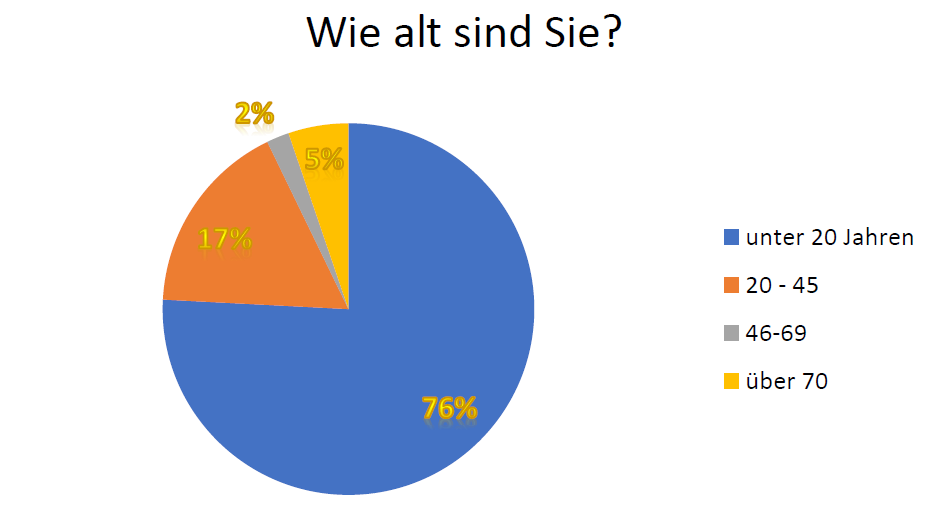
\includegraphics[width=0.8\textwidth]{./img/umfrage1}
	\captionof{figure}{\label{fig:Frage1}Umfrage - Frage 1}
\end{center}
An der Umfrage haben insgesamt 120 Personen teilgenommen. Davon waren 76\% unter 20 Jahren, 17\% 20 bis 45 Jahre, 2\% 46 bis 69 Jahre und 5\% über 70 Jahre alt.

\subsection{Frage 2}
\begin{center}
	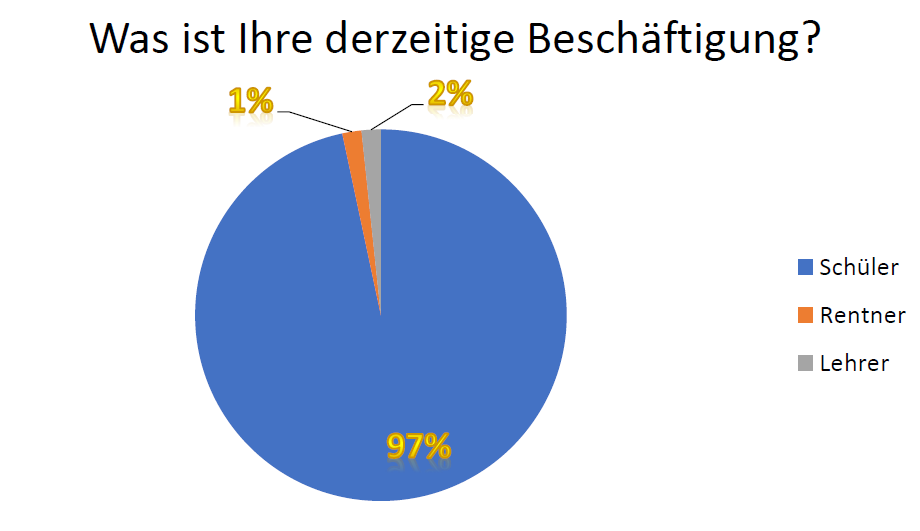
\includegraphics[width=0.8\textwidth]{./img/umfrage2}
	\captionof{figure}{\label{fig:Frage2} Umfrage - Frage 2}
\end{center}
Von den Befragten waren 97\% Schüler, 1\% Rentner und 2\% Lehrer.


\subsection{Frage 3}
\begin{center}
	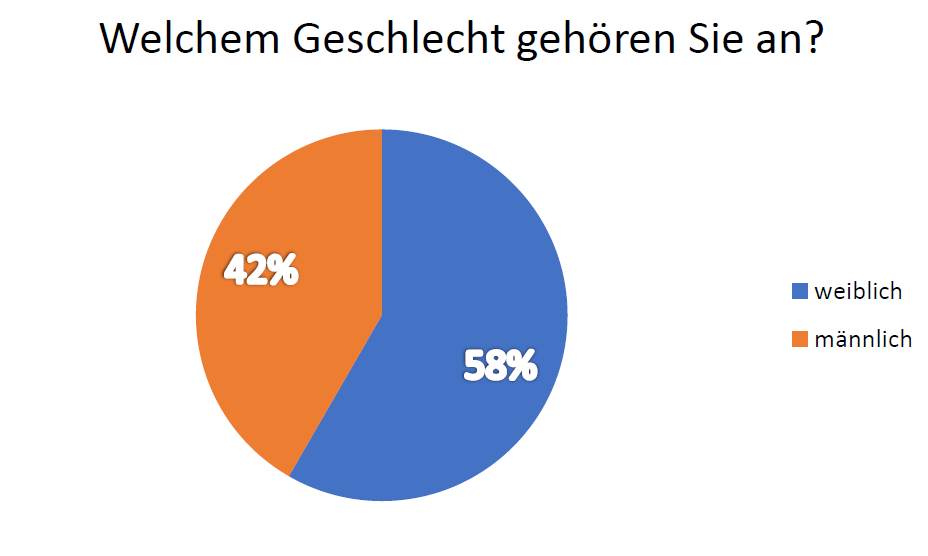
\includegraphics[width=0.8\textwidth]{./img/umfrage3}
	\captionof{figure}{\label{fig:Frage3} Umfrage - Frage 3}
\end{center}
An der Umfrage haben mehr Frauen (58\%) teilgenommen als Männer (42\%).

\subsection{Frage 4}
\begin{center}
	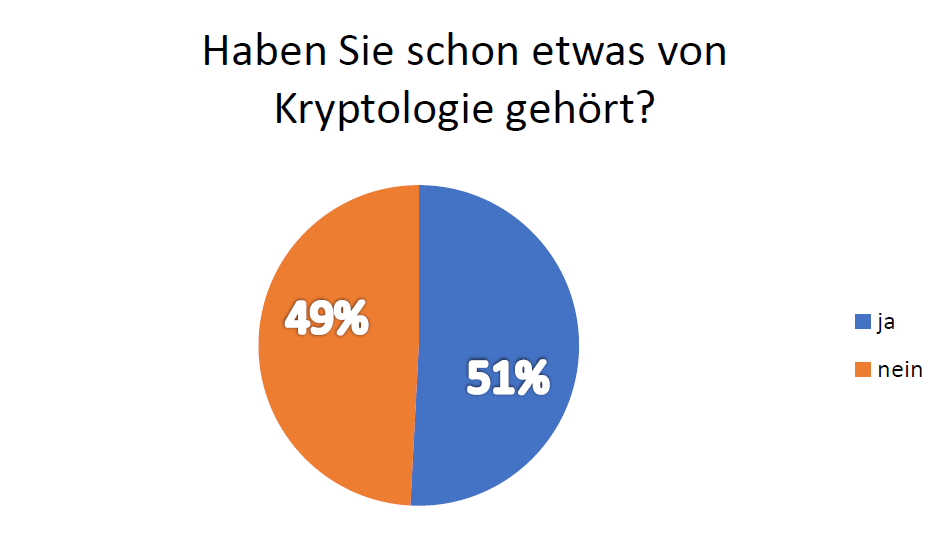
\includegraphics[width=0.8\textwidth]{./img/umfrage4}
	\captionof{figure}{\label{fig:Frage4} Umfrage - Frage 4}
\end{center}
51\% der Personen haben zuvor schon einmal etwas über Kryptologie gehört und 49\% konnten sich darunter nichts vorstellen.

\subsection{Frage 5}
\begin{center}
	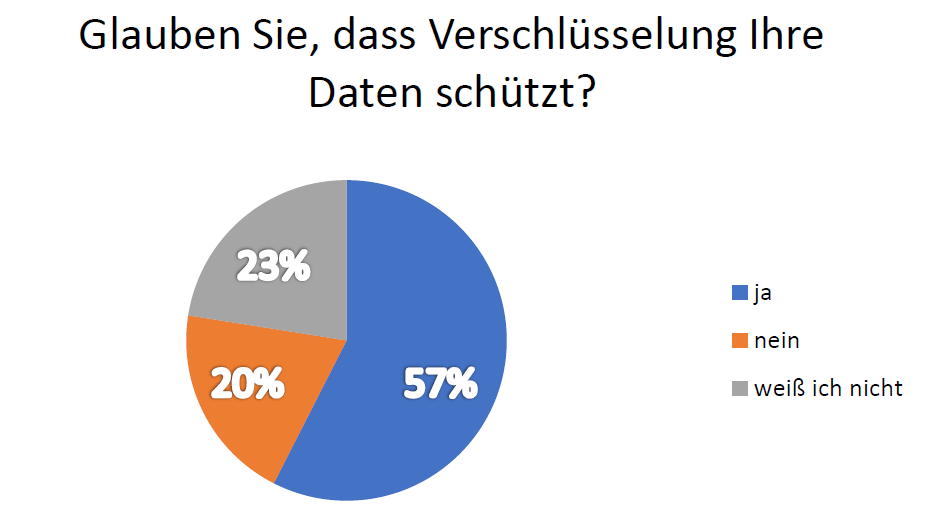
\includegraphics[width=0.8\textwidth]{./img/umfrage5}
	\captionof{figure}{\label{fig:Frage5} Umfrage - Frage 5}
\end{center}
Bei der Umfrage gaben 57\% an, dass eine Verschlüsselung die Daten schützen kann. 20\% glaubten nicht das dies der Fall ist und 23\% gaben an, dass sie das nicht wüssten.


\subsection{Frage 6}
\begin{center}
	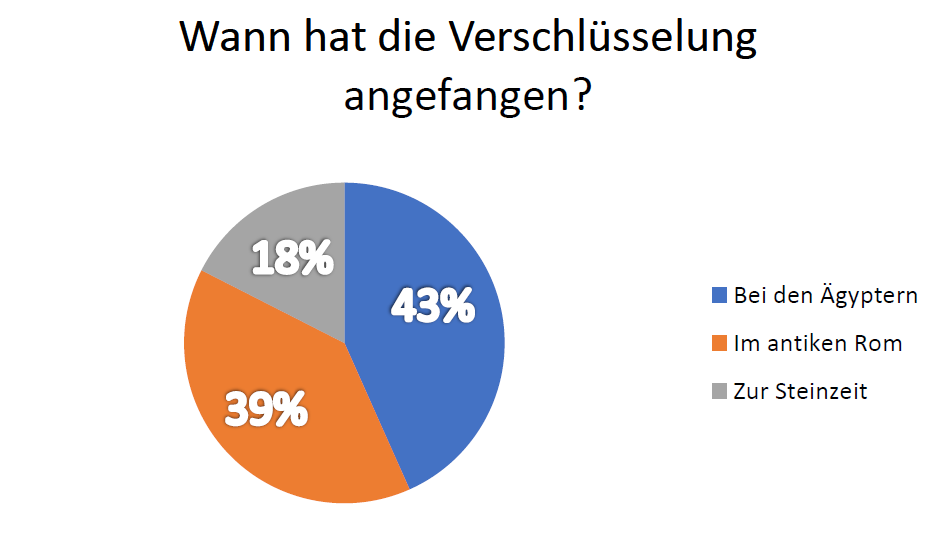
\includegraphics[width=0.8\textwidth]{./img/umfrage6}
	\captionof{figure}{\label{fig:Frage6} Umfrage - Frage 6}
\end{center}
Bei der Frage: Wann hat die Verschlüsselung angefangen gaben 43\% bei den Ägyptern, 39\% im antiken Rom und 18\% zur Steinzeit an.


\subsection{Frage 7}
\begin{center}
	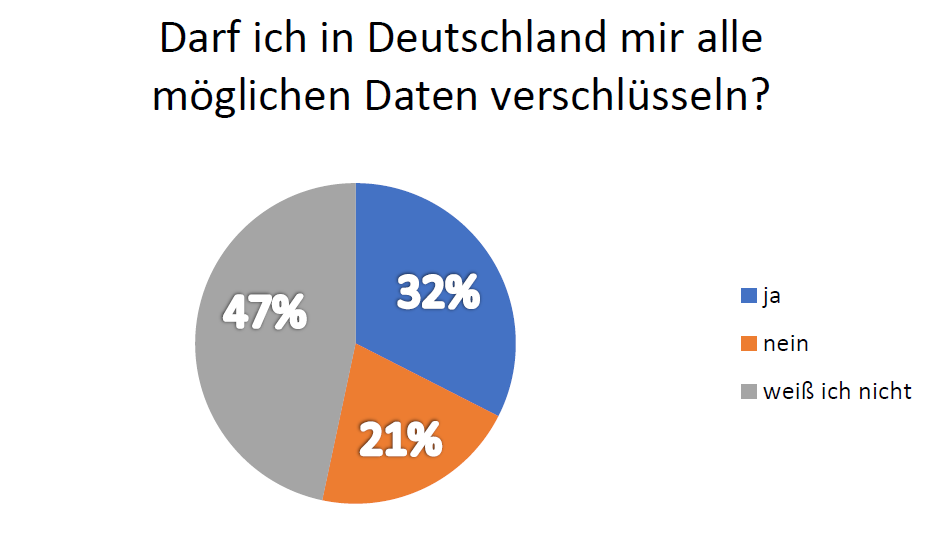
\includegraphics[width=0.8\textwidth]{./img/umfrage7}
	\captionof{figure}{\label{fig:Frage7} Umfrage - Frage 7}
\end{center}
Es gaben 32\% an, dass man alle möglichen Daten in Deutschland verschlüsseln darf. 21\% der Befragten gaben nein an. Und 47\% gaben an, dass Sie nicht darüber wissen.



\subsection{Frage 8}
\begin{center}
	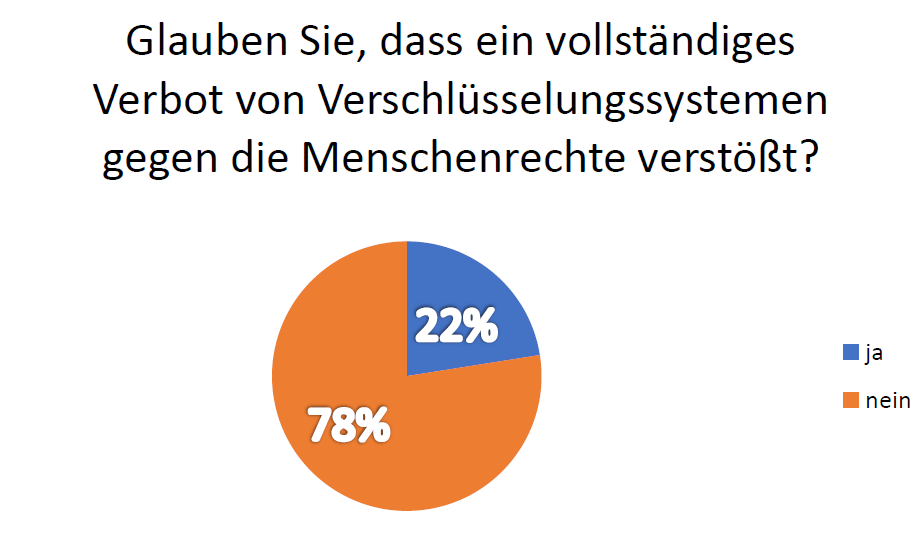
\includegraphics[width=0.8\textwidth]{./img/umfrage8}
	\captionof{figure}{\label{fig:Frage8} Umfrage - Frage 8}
\end{center}
Es gaben 32\% an, dass man alle möglichen Daten in Deutschland verschlüsseln darf. 21\% der Befragten gaben nein an. Und 47\% gaben an, dass Sie nicht darüber wissen.
78\% der Befragten gaben an, dass es nicht gegen die Menschenrechte verstoßen würden und 22\% sagten, dass es gegen die Menschenrechte verstößt.

\subsection{Frage 9}
\begin{center}
	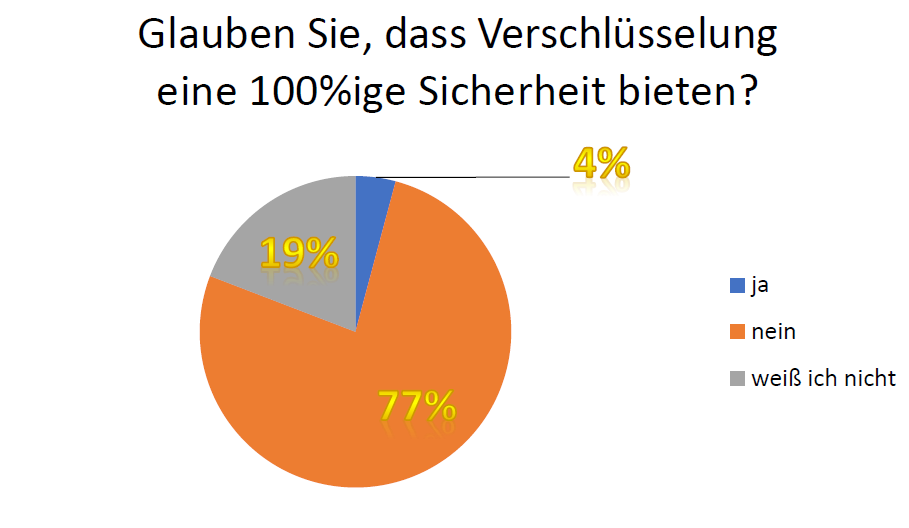
\includegraphics[width=0.8\textwidth]{./img/umfrage9}
	\captionof{figure}{\label{fig:Frage9} Umfrage - Frage 9}
\end{center}
Bei der Frage: Glauben Sie, dass Verschlüsselung eine 100\%ige Sicherheit bieten, gaben 4\% ja, 77\% nein und 19\% weiß ich nicht an.

\subsection{Frage 10}
\begin{center}
	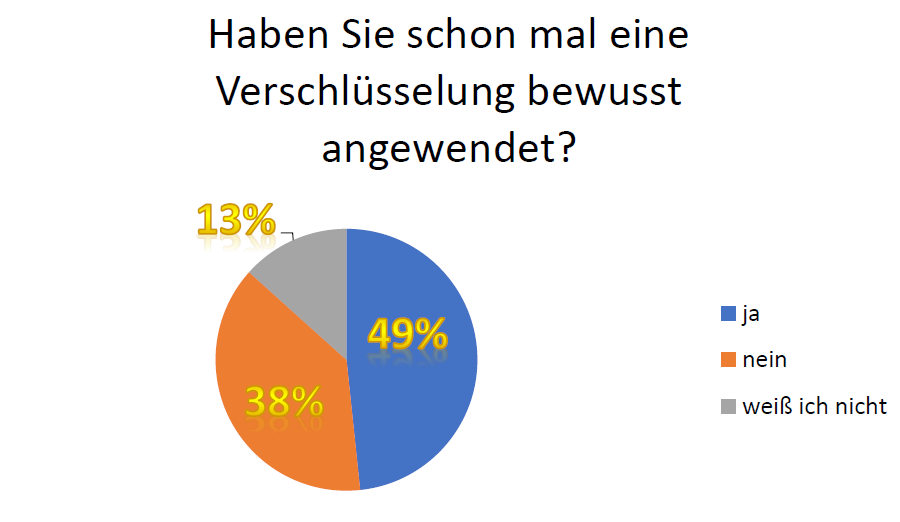
\includegraphics[width=0.8\textwidth]{./img/umfrage10}
	\captionof{figure}{\label{fig:Frage10} Umfrage - Frage 10}
\end{center}
Bei dieser Frage gaben 49\% ja, 38\% nein und 13\% weiß ich nicht an.


%%% Ende %%%

\appendix
\part*{Anhang}


% Anahng
%% ++++++++++++++++++++++++++++++++++++++++++++++++++++++++++++
%% Anhang: Literaturverzeichnis
%% ++++++++++++++++++++++++++++++++++++++++++++++++++++++++++++


% Mit dem Befehl \nocite werden auch nicht im Text zitierte
% aus der Literaturdatenbank mit in das Literaturverzeichnis aufgenommen.
% Ein "\nocite{*}" übernimmt ungeprüft die komplette Datenbank.
%\nocite{*}

\cleardoublepage
\ihead[]{Literaturverzeichnis}
\bibliographystyle{alphadin}
\bibliography{literatur} % "literatur.bib" ist hier die einzige Literaturdatenbank.

% Alternativ: Mehrere Datenbanken verwenden, falls eine
% oder mehrere umfangreiche Sammlungen exisitieren:
%\bibliography{literatur_buecher,literatur_weblinks}


%% ++++++++++++++++++++++++++++++++++++++++++++++++++++++++++++
%% Anhang: Abbildungsverzeichnis
%% ++++++++++++++++++++++++++++++++++++++++++++++++++++++++++++


% Keine Änderungen vornehmen!
\cleardoublepage
\ihead[]{Abbildungsverzeichnis}
\listoffigures


%% ++++++++++++++++++++++++++++++++++++++++++++++++++++++++++++
%% Anhang: Abkürzungsverzeichnis
%% ++++++++++++++++++++++++++++++++++++++++++++++++++++++++++++


% Hier keine weiteren Änderungen vornehmen
\cleardoublepage
\ihead[]{Abkürzungsverzeichnis und Formelzeichen}
\printnomenclature




% Abschlusserklärung
%% ++++++++++++++++++++++++++++++++++++++++++++++++++++++++++++
%% Vorwort: Abschlusserklärung
%% ++++++++++++++++++++++++++++++++++++++++++++++++++++++++++++


\chapter*{Erklärung}
\addcontentsline{toc}{chapter}{Erklärung}
\ihead[]{Erklärung}

Die vorliegende Arbeit habe ich selbstständig ohne Benutzung anderer als der
angegebenen Quellen angefertigt. Alle Stellen, die wörtlich oder sinngemäß
aus veröffentlichten Quellen entnommen wurden, sind als solche
kenntlich gemacht. Die Arbeit ist in gleicher oder ähnlicher Form oder
auszugsweise im Rahmen einer oder anderer Prüfungen noch nicht vorgelegt
worden.
\\[2cm]
Ilmenau, den \today \hfill \namedesautors




\end{document}
